%杨舒云的实验报告编辑界面,使用了Huanyu Shi,2019级的模板,杨舒云在此拜谢ORZ!

%!TEX program = xelatex
\documentclass[dvipsnames, svgnames,a4paper,11pt]{article}
% ----------------------------------------------------- 
%	加边框的命令
%	参考:https://tex.stackexchange.com/questions/531559/how-to-add-the-page-border-for-first-two-pages-in-latex
\usepackage{tikz}
\usetikzlibrary{calc}
\usepackage{eso-pic}
\AddToShipoutPictureBG{%
\begin{tikzpicture}[overlay,remember picture]
\draw[line width=0.6pt] % 边框粗细
    ($ (current page.north west) + (0.6cm,-0.6cm) $)
    rectangle
    ($ (current page.south east) + (-0.6cm,0.6cm) $); % 边框位置
\end{tikzpicture}}


\usepackage{xcolor}
\definecolor{c1}{HTML}{086173} % 目录颜色 原版为2752C9 紫灰色535AAA 蓝紫色0B0DB7 深蓝色070F94 湖绿色219394 松石灰绿086173
\definecolor{c2}{HTML}{E20129} % 引用颜色 原版\definecolor{c2}{RGB}{190,20,83} 橙色F24729

\usepackage{ctex}
\usepackage[top=28mm,bottom=28mm,left=15mm,right=15mm]{geometry}
\usepackage{hyperref} 
\hypersetup{
	colorlinks,
	linktoc = section, % 超链接位置,选项有section, page, all
	linkcolor = c1, % linkcolor 目录颜色
	citecolor = c1  % citecolor 引用颜色
}
\usepackage{amsmath,enumerate,multirow,float}
\usepackage{tabularx}
\usepackage{tabu}
\usepackage{subfig}
\usepackage{fancyhdr}
\usepackage{graphicx}
\usepackage{wrapfig}  
\usepackage{physics}
\usepackage{appendix}
\usepackage{amsfonts}

%
\usepackage{tcolorbox}
\tcbuselibrary{skins,breakable}
\newtcolorbox{tbox}[2][]{
    colframe=black!70!,
    breakable,
    enhanced,
	boxrule =0.5pt,
    title = {#2},
    fonttitle = \large\kaishu\bfseries,
	drop fuzzy shadow,
    #1
}
\newtcolorbox[auto counter,number within=section]{question}[1][]{
  top=2pt,bottom=2pt,arc=1mm,
  boxrule=0.5pt,
%   frame hidden,
  breakable,
  enhanced, %跨页后不会显示下边框
  coltitle=c1!80!gray,
  colframe=c1,
  colback=c1!3!white,
  drop fuzzy shadow,
  title={思考题~\thetcbcounter:\quad},
  fonttitle=\bfseries,
  attach title to upper,
  #1
}

% ---------------------------------------------------------------------
%	利用cleveref改变引用格式,\cref是引用命令
\usepackage{cleveref}
\crefformat{figure}{#2{\textcolor{c2}{Figure #1}}#3} % 图片的引用格式
\crefformat{equation}{#2{(\textcolor{c2}{#1})}#3} % 公式的引用格式
\crefformat{table}{#2{\textcolor{c2}{Table #1}}#3} % 表格的引用格式


% ---------------------------------------------------------------------
%	页眉页脚设置
\fancypagestyle{plain}{\pagestyle{fancy}}
\pagestyle{fancy}
\lhead{\kaishu 中山大学物理与天文学院电子技术实验\uppercase\expandafter{\romannumeral1}} % 左边页眉,学院 + 课程
\rhead{\kaishu 实验报告By杨舒云\&戴鹏辉} % 右边页眉,实验报告标题
\cfoot{\thepage} % 页脚,中间添加页码


% ---------------------------------------------------------------------
%	对目录、章节标题的设置
\renewcommand{\contentsname}{\centerline{\huge 目录}}
\usepackage{titlesec}
\usepackage{titletoc}
% \titleformat{章节}[形状]{格式}{标题序号}{序号与标题间距}{标题前命令}[标题后命令]
\titleformat{\section}{\centering\LARGE\songti}{}{1em}{}

% ---------------------------------------------------------------------
%   listing代码环境设置
\usepackage{listings}
\lstloadlanguages{python}
\lstdefinestyle{pythonstyle}{
backgroundcolor=\color{gray!5},
language=python,
frameround=tftt,
frame=shadowbox, 
keepspaces=true,
breaklines,
columns=spaceflexible,                   
basicstyle=\ttfamily\small, % 基本文本设置,字体为teletype,大小为scriptsize
keywordstyle=[1]\color{c1}\bfseries, 
keywordstyle=[2]\color{Red!70!black},   
stringstyle=\color{Purple},       
showstringspaces=false,
commentstyle=\ttfamily\scriptsize\color{green!40!black},%注释文本设置,字体为sf,大小为smaller
tabsize=2,
morekeywords={as},
morekeywords=[2]{np, plt, sp},
numbers=left, % 代码行数
numberstyle=\it\tiny\color{gray}, % 代码行数的数字字体设置
stepnumber=1,
rulesepcolor=\color{gray!30!white}
}




% ---------------------------------------------------------------------
%	其他设置
\def\degree{${}^{\circ}$} % 角度
\graphicspath{{./images/}} % 插入图片的相对路径
\allowdisplaybreaks[4]  %允许公式跨页 
\usepackage{lipsum}
\usepackage{adjustbox}
%\usepackage{mathrsfs} % 字体
\captionsetup[figure]{name=Figure} % 图片形式
\captionsetup[table]{name=Table} % 表格形式v
\usepackage{tabularray}


\begin{document}
	
	
	
	% 实验报告封面	
	
	% 顶栏
	\begin{table}
		\renewcommand\arraystretch{1.7}
		\begin{tabularx}{\textwidth}{
				|X|X|X|X
				|X|X|X|X|}
			\hline
			\multicolumn{2}{|c|}{预习报告}&\multicolumn{2}{|c|}{实验记录}&\multicolumn{2}{|c|}{分析讨论}&\multicolumn{2}{|c|}{总成绩}\\
			\hline
			\LARGE25 & & \LARGE25 & & \LARGE30 & & \LARGE80 & \\
			\hline
		\end{tabularx}
	\end{table}
	% ---
	
	% 信息栏
	\begin{table}
		\renewcommand\arraystretch{1.7}
		\begin{tabularx}{\textwidth}{|X|X|X|X|}
			\hline
			年级、专业: & 2022级 物理学 &组号: & 2\\
			\hline
			姓名: & 戴鹏辉、杨舒云  & 学号: & 22344016、22344020\\
			\hline
			实验时间: & 2024/6/12 & 教师签名: & \\
			\hline
		\end{tabularx}
	\end{table}
	% ---
	
	% 大标题
	\begin{center}
		\LARGE ET1-13 \quad 整流滤波与稳压电路
	\end{center}
	% ---
	
	% 注意事项
	
	% 基本
	\textbf{【实验报告注意事项】}
	\begin{enumerate}
		\item 实验报告由三部分组成:
		\begin{enumerate}
			\item 预习报告:课前认真研读实验讲义,弄清实验原理;实验所需的仪器设备、用具及其使用、完成课前预习思考题;了解实验需要测量的物理量,并根据要求提前准备实验记录表格(可以参考实验报告模板,可以打印)。\textcolor{red}{\textbf{(20分)}}
			\item 实验记录:认真、客观记录实验条件、实验过程中的现象以及数据。实验记录请用珠笔或者钢笔书写并签名(\textcolor{red}{\textbf{用铅笔记录的被认为无效}})。\textcolor{red}{\textbf{保持原始记录,包括写错删除部分,如因误记需要修改记录,必须按规范修改。}}(不得输入电脑打印,但可扫描手记后打印扫描件);离开前请实验教师检查记录并签名。\textcolor{red}{\textbf{(30分)}}
			\item 数据处理及分析讨论:处理实验原始数据(学习仪器使用类型的实验除外),对数据的可靠性和合理性进行分析;按规范呈现数据和结果(图、表),包括数据、图表按顺序编号及其引用;分析物理现象(含回答实验思考题,写出问题思考过程,必要时按规范引用数据);最后得出结论。\textcolor{red}{\textbf{(30分)}}
		\end{enumerate}
		\textbf{实验报告就是将预习报告、实验记录、和数据处理与分析合起来,加上本页封面。\textcolor{red}{(80分)}}
		\item 每次完成实验后的一周内交\textbf{实验报告}(特殊情况不能超过两周)。
		\item \textbf{其它注意事项}:
		\begin{enumerate}
			\item 由于变压器输出没有限流保护,接线时要注意不要短路;
			\item 用示波器测量时,注意两个通道探头的地线要共地;
			\item 用示波器测量纹波大小时,可以先采用直流耦合,获取直流分量的平均值,再采用交流耦合,观测纹波的波动范围;
			\item 选择和调节负载电阻时,注意不要使负载电流过大;
		\end{enumerate}
	\end{enumerate}
	
	% 安全
	%\textbf{【实验安全注意事项】}	
	
	
	% ---
	
	% 特别鸣谢
	\textbf{【特别鸣谢及模板说明】}	
	
	感谢2019级学长石寰宇为本实验报告提供\LaTeX 模板。\textcolor{red}{\textbf{由于原实验报告模板缺少实验编号,为方便在电脑上整理,故添加自命名编号ET1-11。}}
	% ---
	
	
	
	% 目录
	\clearpage
	\tableofcontents
	\clearpage
	% ---
	
	
	
	% 预习报告	
	
	% 小标题
	\setcounter{section}{0}
	\section{ET1-13 整流滤波与稳压电路 \quad\heiti 预习报告}
	% ---
	
	% 实验目的
	\subsection{实验目的}
	\begin{enumerate}
		\item 比较半波整流与桥式整流的特点。
		\item 了解稳压电路的组成和稳压作用。
		\item 熟悉集成三端可调稳压器的使用。
		\item 掌握直流稳压电源主要参数测试方法。 		
	\end{enumerate}
	% ---
	

	
	% 仪器用具
	\subsection{仪器用具}
	\begin{table}[htbp]
		\centering
		\renewcommand\arraystretch{1.6}
		% \setlength{\tabcolsep}{10mm}
		\begin{tabular}{p{0.05\textwidth}|p{0.20\textwidth}|p{0.05\textwidth}|p{0.5\textwidth}}
			\hline
			编号& 仪器用具名称 & 数量 &  主要参数(型号,测量范围,测量精度等) \\
			\hline
			1&  电路原理箱或板& 1 &  \\
			\hline
			2&  函数信号发生器& 1 &  \\
			\hline
			3&  交流毫伏表& 1 &  \\
			\hline
			4&  数字万用表& 1 &  \\
			\hline
			5&  双踪示波器& 1 &  \\
			\hline
		\end{tabular}
	\end{table}
	% ---
	
	% 原理概述
	\subsection{原理概述}

		\subsubsection*{半波整流和全波整流的电路结构与形式}

			\begin{itemize}
				\item 半波整流
				
				\begin{figure}[htbp]
					\centering
					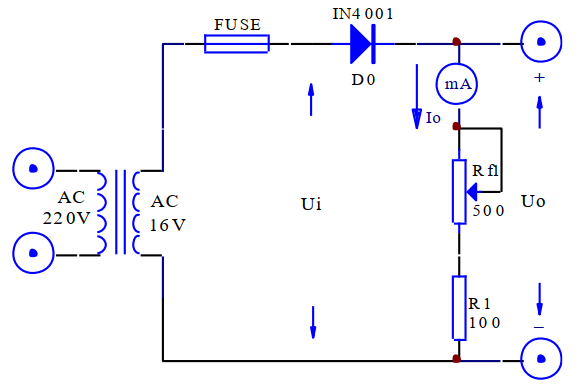
\includegraphics[width=0.4\textwidth]{ET1_13Gra1-1.png}
					\caption{半波整流电路示意图}
					\label{fig:figP1}
				\end{figure}

				半波整流电路通常由一个二极管和一个负载电阻组成。其工作原理为:

				\begin{enumerate}
					\item 正半周期:当输入交流电的正半周期时,二极管正向偏置(阳极电压高于阴极电压),导通,交流电压通过二极管和负载电阻,输出电压等于输入电压的正半周期波形。
					\item 负半周期:当输入交流电的负半周期时,二极管反向偏置(阳极电压低于阴极电压),截止,电流无法通过,输出电压为零。
	
				\end{enumerate}
			
				因此,半波整流只利用了输入电压的正半周期,输出电压为单极性脉动直流电,包含大量的交流分量。


				\item 全波整流
				
				\begin{figure}[htbp]
					\centering
					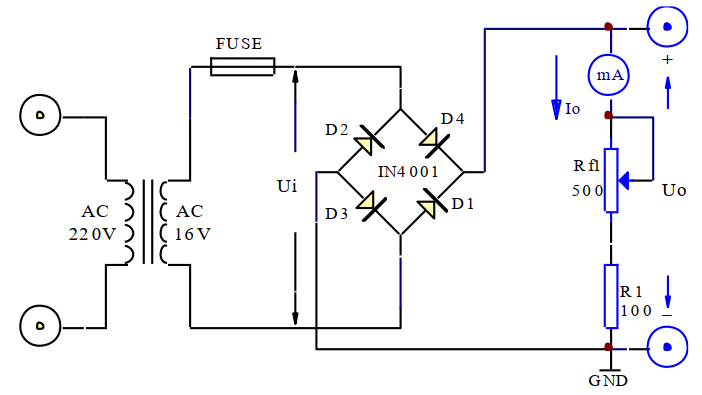
\includegraphics[width=0.4\textwidth]{ET1_13Gra1-2.png}
					\caption{全波整流电路示意图}
					\label{fig:figP1}
				\end{figure}


				桥式整流电路由四个二极管组成一个桥式整流器,其工作原理为:

				\begin{enumerate}
					\item 正半周期:在输入交流电的正半周期时,D1和D2二极管正向偏置,导通;D3和D4二极管反向偏置,截止。电流通过D1、负载电阻、D2流动,输出正的半波。
					\item 负半周期:在输入交流电的负半周期时,D3和D4二极管正向偏置,导通;D1和D2二极管反向偏置,截止。电流通过D3、负载电阻、D4流动,输出也是正的半波。
				\end{enumerate}
				
				桥式整流利用了输入电压的两个半周期,输出电压为双极性脉动直流电。
			\end{itemize}
			
		\subsubsection*{RC一阶电路时间常数对电容放电曲线的影响}

			$RC$一阶电路由一个电阻 $R$ 和一个电容 $C$ 串联组成,时间常数$\tau$定义为电阻 $R$ 和电容 $C$ 的乘积。时间常数 $\tau$ 表示电容电压在放电过程中下降至初始值的$1/e$(大约36.8\%)所需的时间。

			电容在放电过程中,电压 V(t) 随时间 t 的变化可以用指数函数表示:

			\[
				V(t) = V_0 e^{-\frac{t}{\tau}}
			\]
		
			时间常数对放电曲线有一定的影响:
			\begin{enumerate}
				\item 较小的时间常数:
				
				当时间常数 $\tau$ 较小时,电容的放电速度较快。这意味着电容电压会迅速下降到接近于零。在图形上表现为放电曲线陡峭。

				\item 较大的时间常数:
				
				当时间常数 $\tau$ 较大时,电容的放电速度较慢。这意味着电容电压会缓慢下降。在图形上表现为放电曲线平缓。

			\end{enumerate}







		\subsubsection*{稳压二极管特性}


			稳压二极管(也称为齐纳二极管)是一种具有特殊特性的半导体器件,广泛应用于电压稳压、过电压保护和电压基准等电路中。

			\begin{itemize}
				\item 稳压二极管的基本概念

					稳压二极管是一种专门设计用于反向击穿模式下稳定电压的二极管。当其反向电压达到特定值(称为齐纳击穿电压)时,二极管开始导通,并在此电压附近保持稳定。

				\item 稳压二极管的特性
				
					\begin{enumerate}
						\item 反向击穿电压(齐纳电压)
						
							反向击穿电压$V_z$是指稳压二极管在反向偏置下开始导通并保持电压稳定的电压值。齐纳电压是稳压二极管最重要的参数之一,不同型号的稳压二极管具有不同的齐纳电压,通常在2V到200V之间。

						\item  齐纳电流$I_z$
						
							齐纳电流是指稳压二极管在反向击穿状态下的工作电流。齐纳电流的大小取决于外部电路中的电阻和输入电压。稳压二极管的工作电流范围一般由制造商给出,包括最小工作电流和最大工作电流。

						\item 齐纳阻抗$Z_z$
						
							齐纳阻抗是指稳压二极管在工作电流范围内的动态电阻。它反映了二极管在不同电流条件下电压变化的幅度。较低的齐纳阻抗意味着更稳定的输出电压。

					
					\end{enumerate}

				\item 稳压二极管的工作原理
					
					稳压二极管在正向偏置下的行为与普通二极管相似,但在反向偏置时具有独特的击穿特性。当反向电压低于齐纳电压时,二极管基本不导通;当反向电压达到齐纳电压时,二极管进入击穿区,反向电流迅速增加,但电压基本保持不变。
			\end{itemize}








		\subsubsection*{电源效率的计算方法}

			电源效率是衡量电源性能的重要指标,它表示电源将输入电能转换为输出电能的有效程度。电源效率的计算方法涉及多个步骤和概念。以下是电源效率计算的详细介绍:

			\begin{itemize}
				\item 电源效率的基本定义:
					
					电源效率$eta$是输出功率$P_{out}$与输入功率$P_{out}$的比值,通常以百分比表示:

					\[
						\eta = \frac{P_{out}}{P_{out}} \times 100\%
					\]

				\item 输入功率和输出功率的计算:
				
					\begin{enumerate}
						\item 输入功率:
						
							输入功率是电源从输入端吸收的总电功率。对于直流电源,输入功率计算较为简单:
							\[
								p_{in} = V_{in}I_{in}
							\]
		
							对于交流电源,还需要考虑功率因数(PF)
							\[
								p_{in} = V_{in}I_{in} \times PF
							\]

						
						\item 输出功率:
						
							输出功率是电源在输出端提供的有效电功率。对于直流电源:
							\[
								p_{out} = V_{out}I_{out}
							\]
		
							对于交流电源,还需要考虑功率因数(PF)
							\[
								p_{out} = V_{out}I_{out} \times PF
							\]

						
					\end{enumerate}
					
				
				\item 电源效率的影响因素
				
					\begin{enumerate}
						\item 转换损耗:电源内部元件如变压器、电感、电容等在能量转换过程中会产生损耗,影响效率。
						\item 温度:高温会增加电源元件的电阻,导致更高的能量损耗。
						\item 负载条件:不同负载条件下电源的效率不同,通常在额定负载下效率最高。
						\item 电源设计:电源电路设计和元件选择直接影响效率,如使用高效的开关元件和低损耗的电感器等。
					\end{enumerate}
				
				\item 提高电源效率的方法
				
					\begin{enumerate}
						\item 优化电源设计:使用高效元件和先进的电路拓扑结构,如同步整流、软开关技术等。
						\item 降低损耗:使用低损耗材料和减少电源内部元件的电阻。
						\item 热管理:通过散热器、风扇和液冷等手段有效管理电源内部温度,减少热损耗。
						\item 功率因数校正:特别是对于交流电源,使用功率因数校正电路提高输入电能的利用率。
					\end{enumerate}

			\end{itemize}



		\subsubsection*{对稳压效果的评估方法,负载调整率如何测试与计算}

		\noindent 对稳压电源的稳压效果进行评估,通常需要考虑两个重要的指标:\textbf{负载调整率}和\textbf{线路调整率}。这两者帮助我们理解电源在不同负载和输入电压条件下的性能。以下是详细介绍这两个评估方法,以及如何测试和计算负载调整率。

		\begin{enumerate}
			\item \textbf{稳压效果的评估方法}
			\begin{enumerate}
				\item \textbf{负载调整率(Load Regulation)}
		
				负载调整率描述的是当输入电压保持恒定时,输出电压随负载变化的程度。它通常表示为输出电压的变化量占初始输出电压的百分比。
		
				负载调整率的计算公式为:
				\[
				\text{负载调整率} = \left( \frac{V_{\text{满载}} - V_{\text{空载}}}{V_{\text{空载}}} \right) \times 100\%
				\]
				其中:
				\begin{itemize}
					\item \(V_{\text{满载}}\) 是电源在最大负载电流时的输出电压。
					\item \(V_{\text{空载}}\) 是电源在最小负载电流(通常为零负载)时的输出电压。
				\end{itemize}
		
				\item \textbf{线路调整率(Line Regulation)}
		
				线路调整率描述的是当负载保持恒定时,输出电压随输入电压变化的程度。它通常表示为输出电压的变化量占初始输出电压的百分比。
		
				线路调整率的计算公式为:
				\[
				\text{线路调整率} = \left( \frac{V_{\text{高}} - V_{\text{低}}}{V_{\text{标称}}} \right) \times 100\%
				\]
				其中:
				\begin{itemize}
					\item \(V_{\text{高}}\) 是在最高输入电压时的输出电压。
					\item \(V_{\text{低}}\) 是在最低输入电压时的输出电压。
					\item \(V_{\text{标称}}\) 是标称输入电压时的输出电压。
				\end{itemize}
			\end{enumerate}
		
			\item \textbf{负载调整率的测试方法}
		
			测试负载调整率的步骤如下:
		
			\begin{enumerate}
				\item \textbf{设定空载条件}
		
				将电源在无负载或最小负载电流的条件下运行,测量并记录输出电压 \(V_{\text{空载}}\)。
		
				\item \textbf{设定满载条件}
		
				将电源连接到最大额定负载,测量并记录输出电压 \(V_{\text{满载}}\)。
		
				\item \textbf{计算负载调整率}
		
				使用前述公式计算负载调整率。
		
				
			\end{enumerate}
		
			\item \textbf{稳压效果的综合评估}
		
			除了负载调整率和线路调整率外,还可以考虑以下几个方面:
		
			\begin{enumerate}
				\item \textbf{纹波和噪声(Ripple and Noise)}
		
				测量输出电压中的纹波和噪声,以评估电源的稳定性和纯净度。使用示波器来观察和测量纹波和噪声电压的峰峰值或均方根值(rms)。
		
				\item \textbf{瞬态响应(Transient Response)}
		
				评估电源在负载突然变化时输出电压的恢复时间和幅度。测试方法通常是在负载电流突然从低值跃升至高值或从高值下降至低值时,观察和记录输出电压的变化。
		
				\item \textbf{温度稳定性(Temperature Stability)}
		
				在不同温度条件下,测量并比较输出电压,以评估电源的温度稳定性。
			\end{enumerate}
		
			
		\end{enumerate}
	% ---
	
	
	
	% 实验前思考题
	%\subsection{实验预习题}
	
	
	
	% ---
	
	
	
	% 实验记录	
	\clearpage
	
	% 顶栏
	\begin{table}
		\renewcommand\arraystretch{1.7}
		\centering
		\begin{tabularx}{\textwidth}{|X|X|X|X|}
			\hline
			专业: & 物理学 & 年级: & 2022级 \\
			\hline
			姓名: & 戴鹏辉、杨舒云 & 学号: & 22344016、22344020\\
			\hline
			室温: & 26\degree C & 实验地点: & A522 \\
			\hline
			学生签名:& 见\textbf{附件}部分 & 评分: &\\
			\hline
			实验时间:& 2024/6/12 & 教师签名:&\\
			\hline
		\end{tabularx}
	\end{table}
	% ---
	
	% 小标题
	\section{ET1-13 整流滤波与稳压电路  \quad\heiti 实验记录}
	% ---
	
	% 实验过程记录
	\subsection{实验内容、步骤与结果}
	
	%
	\subsubsection{操作步骤记录}

		\begin{enumerate}
			\item 搭建半波整流电路,用示波器观测和记录输出波形;
			
				\begin{figure}[htbp]
					\centering
					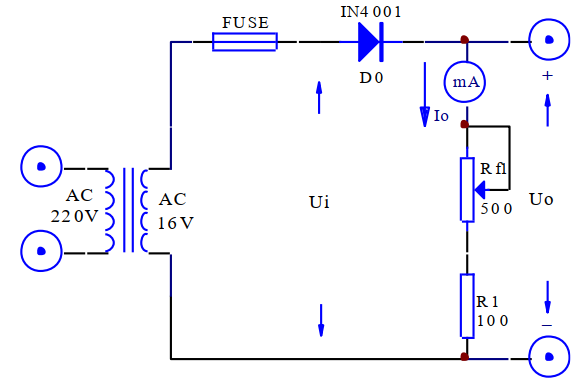
\includegraphics[width=0.4\textwidth]{半波整流电路图.png}
					\caption{半波整流电路图}
					\label{fig:半波整流电路图}
				\end{figure}

				按照电路图\cref{fig:半波整流电路图}连接电路后,得到的输出波形如图\cref{fig:半波整流}所示:

				\begin{figure}[htbp]
					\centering
					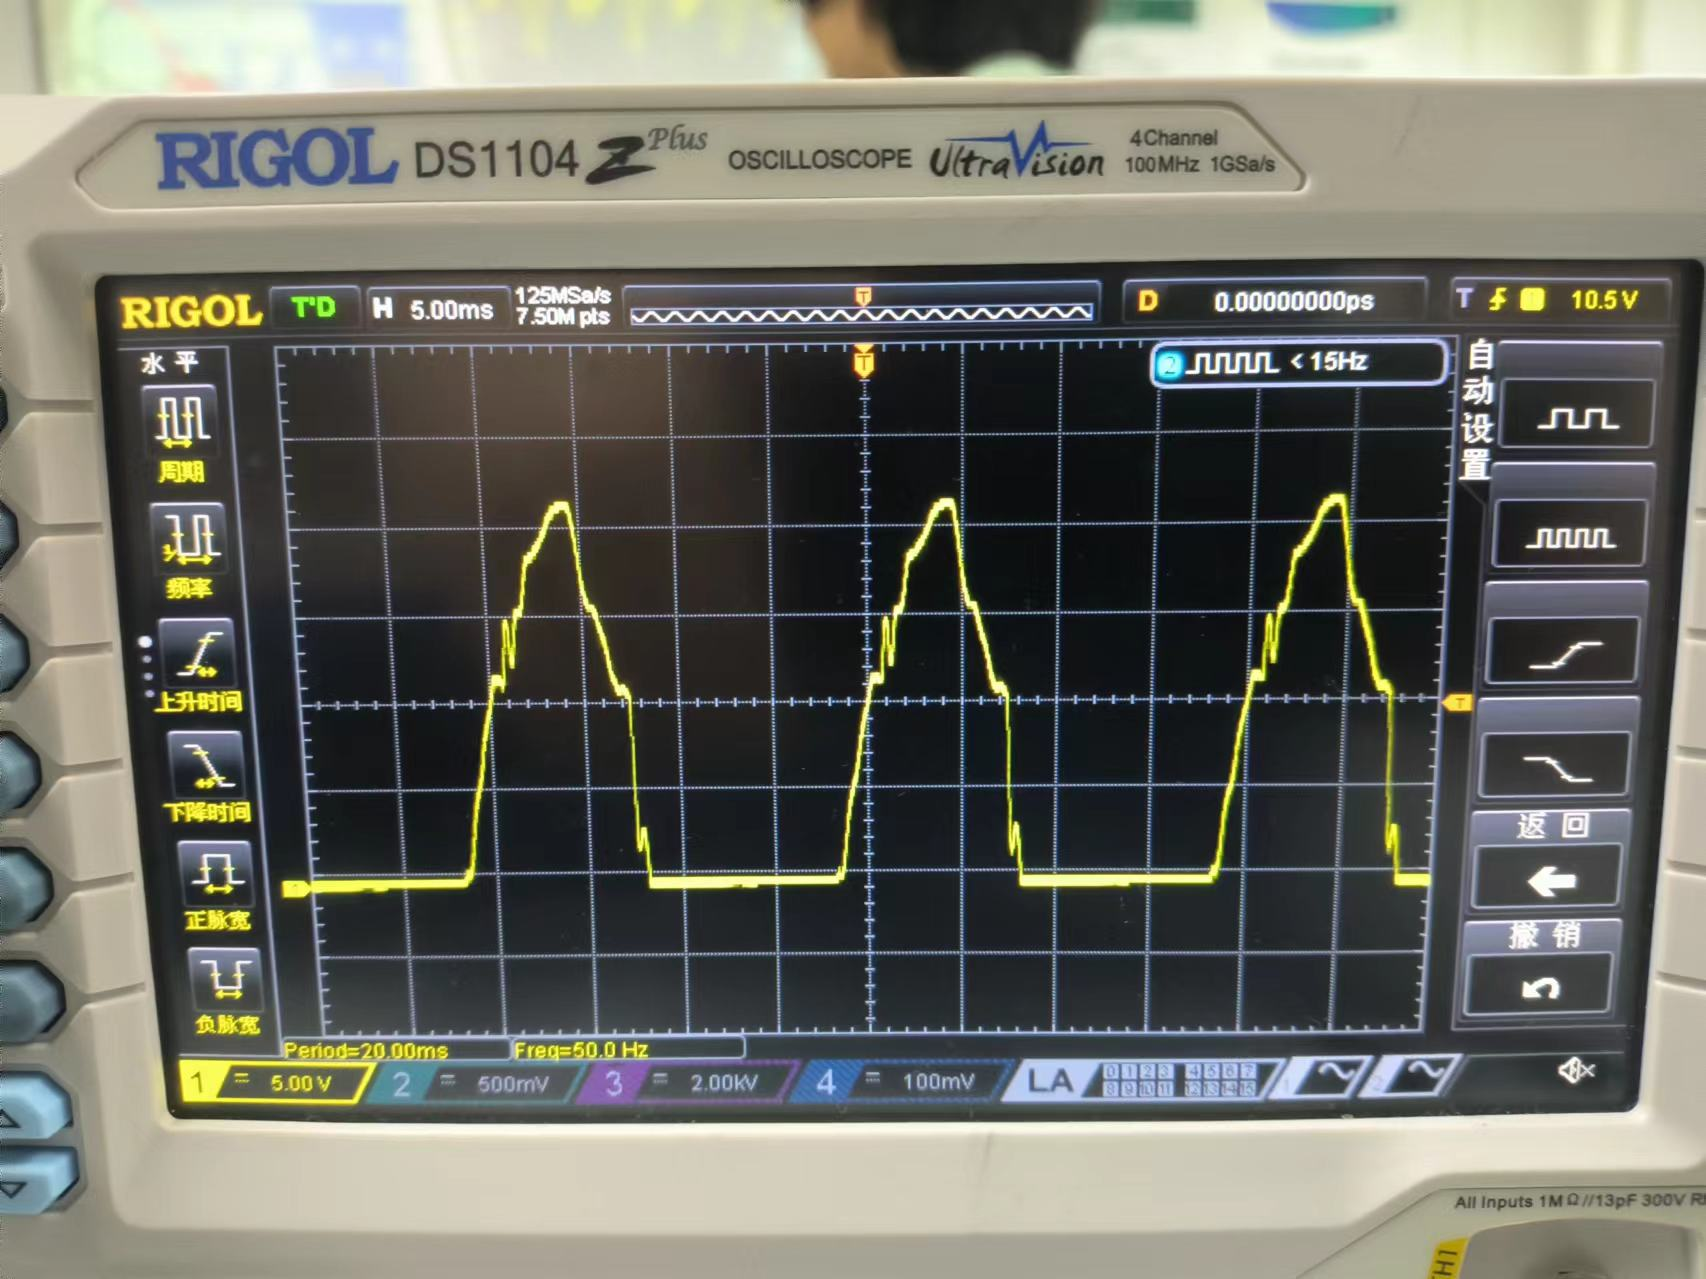
\includegraphics[width=0.4\textwidth]{半波整流效果.jpg}
					\caption{半波整流电路输出波形图}
					\label{fig:半波整流}
				\end{figure}





			\item 搭建桥式整流电路, 用示波器观测和记录输出波形;
			
				\begin{figure}[htbp]
					\centering
					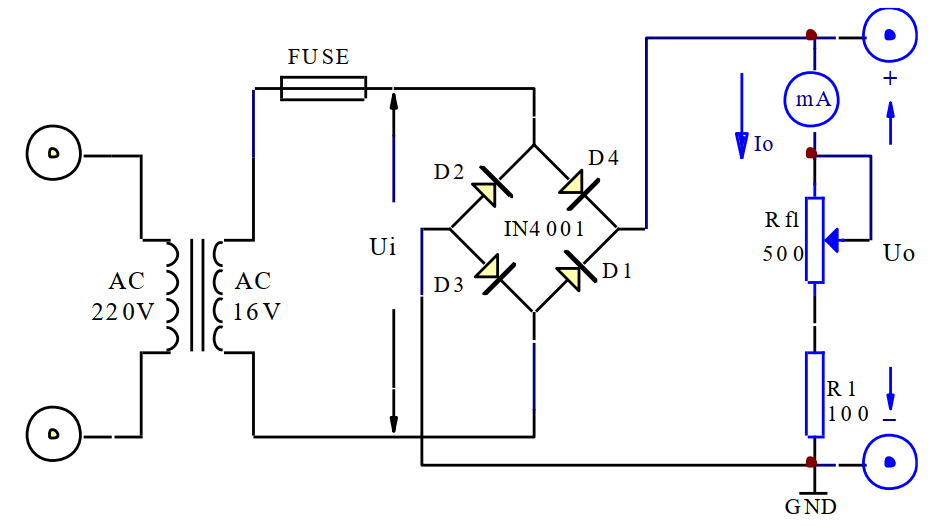
\includegraphics[width=0.4\textwidth]{桥式全波整流电路图.png}
					\caption{桥式全波整流电路图}
					\label{fig:桥式全波整流电路图}
				\end{figure}


				按照电路图\cref{fig:桥式全波整流电路图}连接电路后,得到的输出波形如图\cref{fig:全波整流}所示:


				\begin{figure}[htbp]
					\centering
					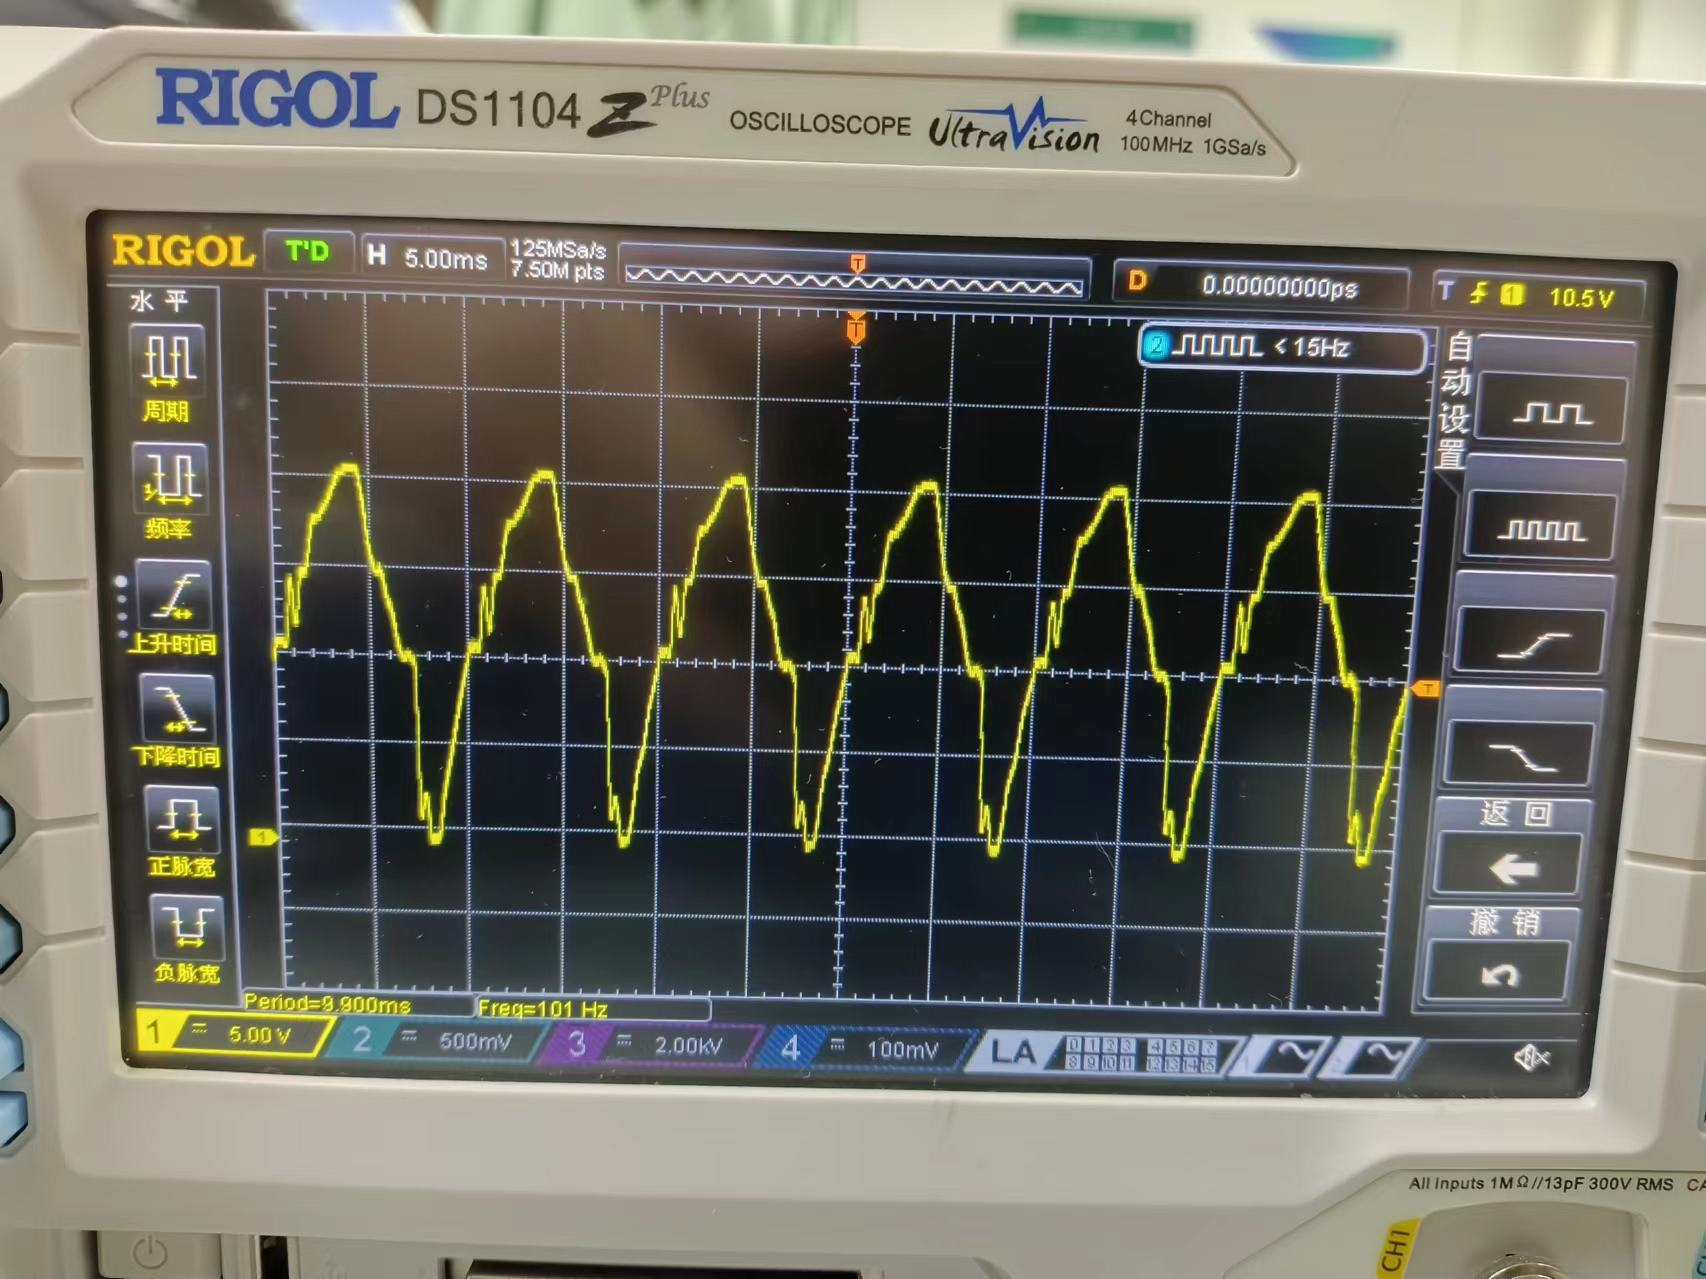
\includegraphics[width=0.4\textwidth]{桥式全波整流效果.jpg}
					\caption{桥式全波整流电路输出波形图}
					\label{fig:全波整流}
				\end{figure}







			\item 加入滤波电容
			
				\begin{figure}[htbp]
					\centering
					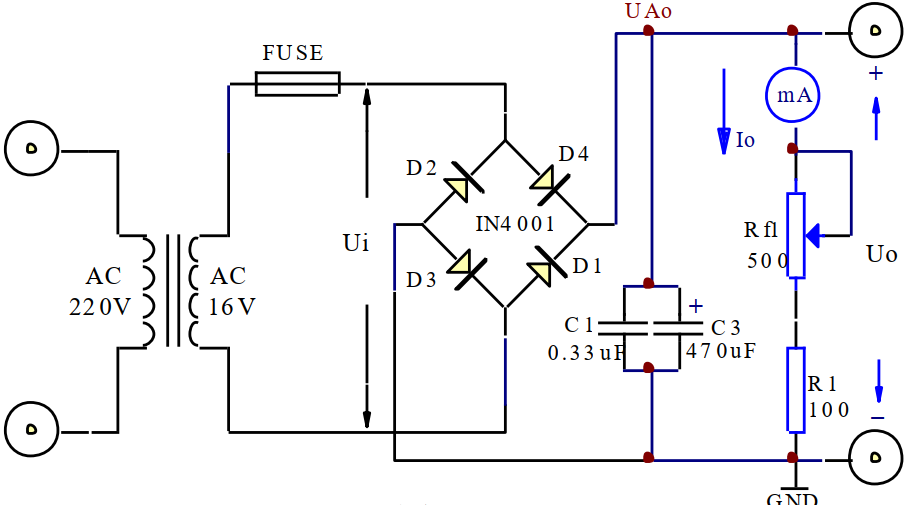
\includegraphics[width=0.4\textwidth]{滤波电容电路图.png}
					\caption{滤波电容电路图}
					\label{fig:滤波电容电路图}
				\end{figure}


				在刚刚全波桥式整流电路的基础上,按照电路图\cref{fig:滤波电容电路图}连接电路,加入滤波电容,得到的结果如\cref{fig:全波整流+滤波电容1}、\cref{fig:全波整流+滤波电容2}所示:

				\begin{figure}[htbp]
					\centering
					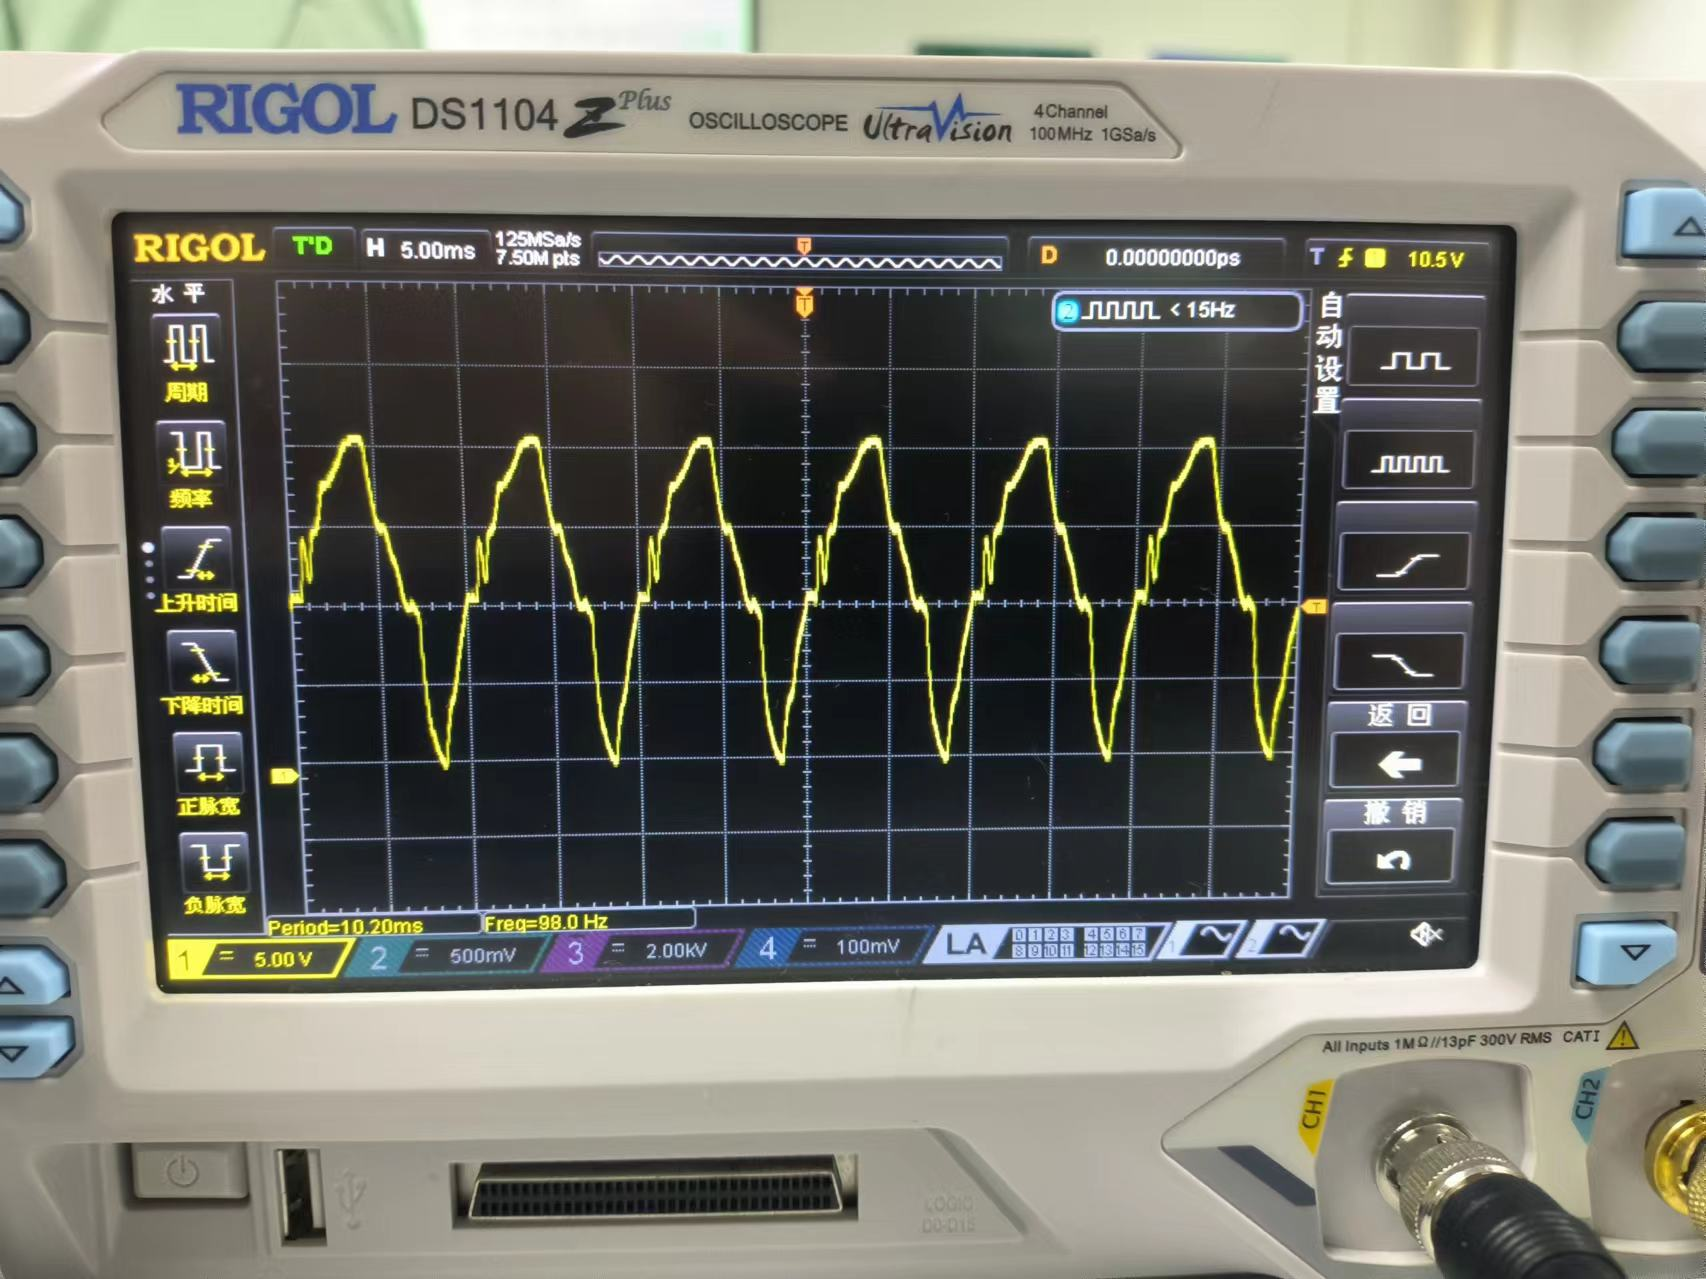
\includegraphics[width=0.4\textwidth]{滤波电容0.33muF.jpg}
					\caption{桥式全波整流电路加入滤波电容0.33$\mu F$}
					\label{fig:全波整流+滤波电容1}
				\end{figure}


				\begin{figure}[htbp]
					\centering
					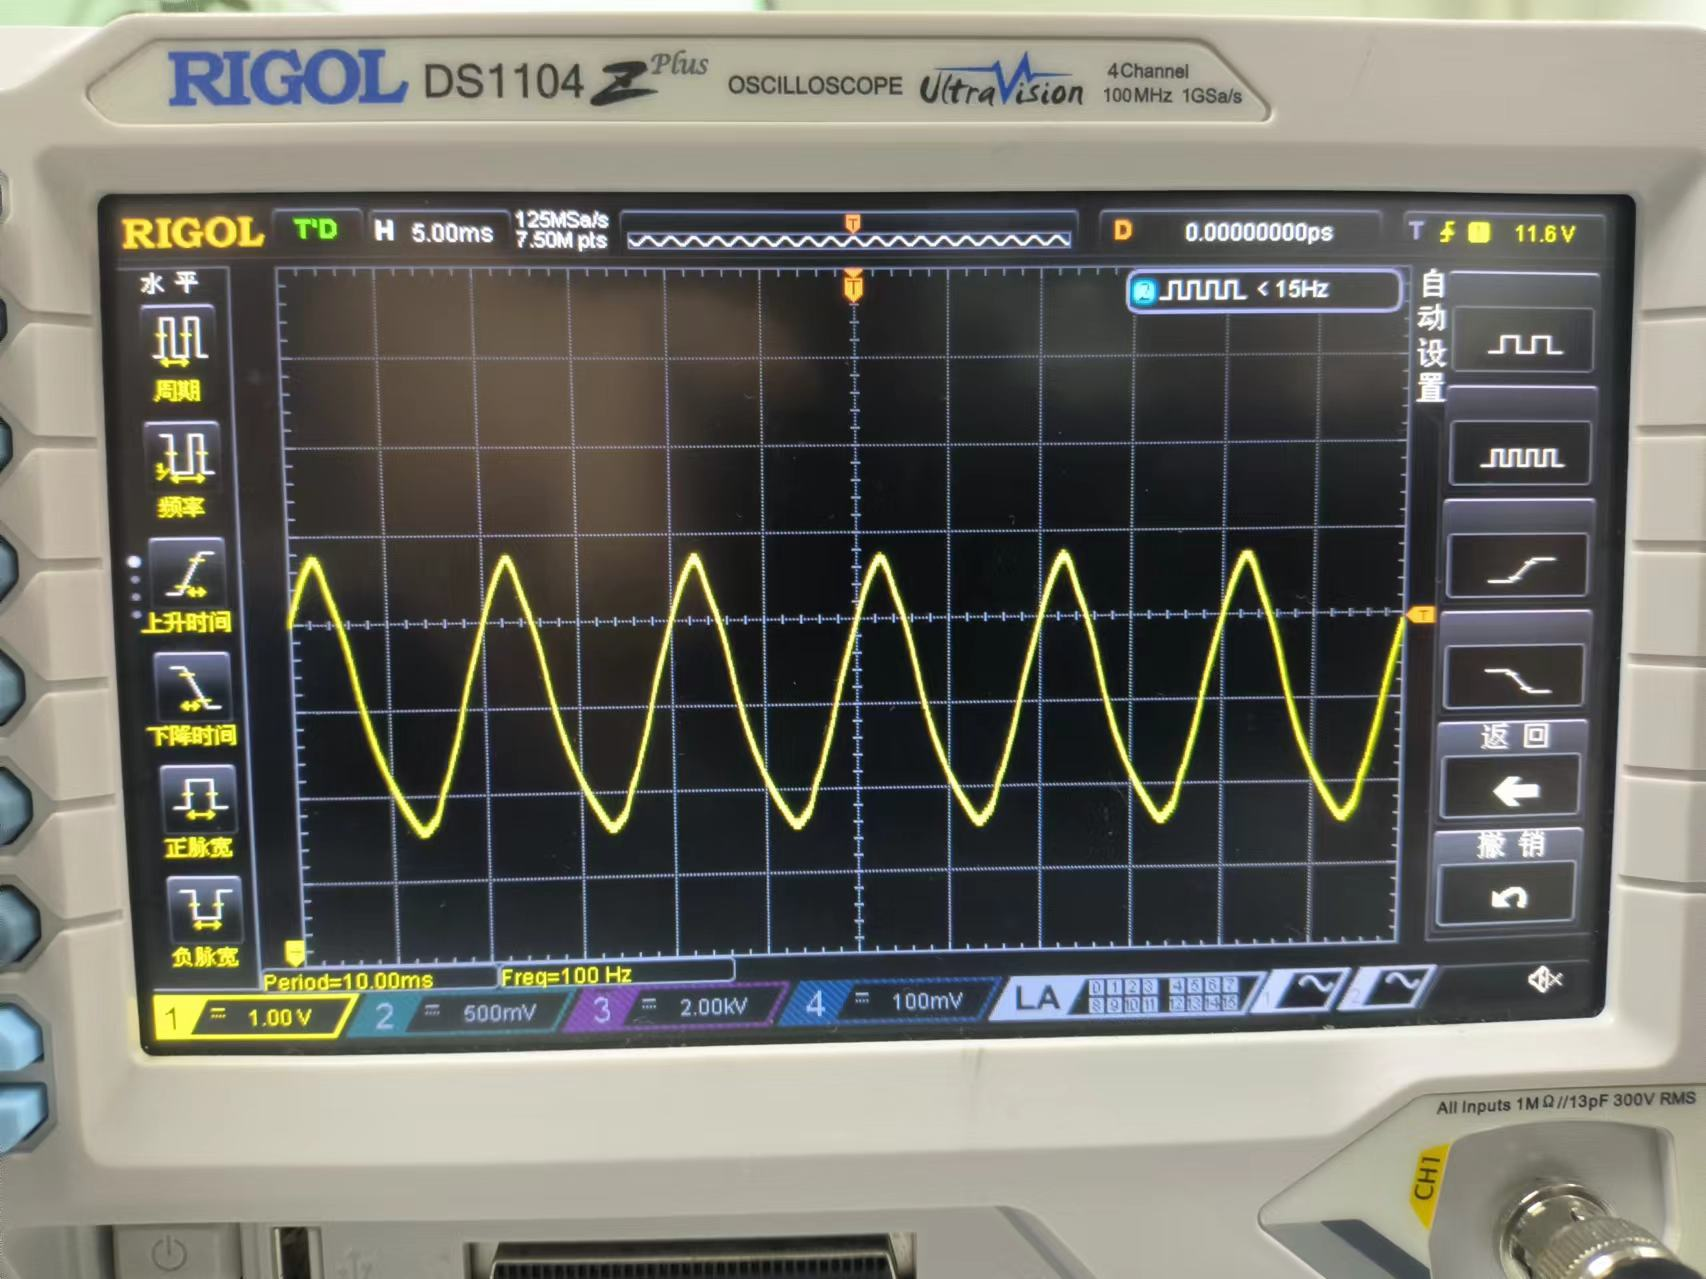
\includegraphics[width=0.4\textwidth]{滤波电容470muF.jpg}
					\caption{桥式全波整流电路加入滤波电容470$\mu F$}
					\label{fig:全波整流+滤波电容2}
				\end{figure}








			\item 在桥式整流滤波电路中,搭建稳压管并联稳压电路,调整负载大小 ,观测并记录稳压电路的稳压效果;
			

				\begin{figure}[htbp]
					\centering
					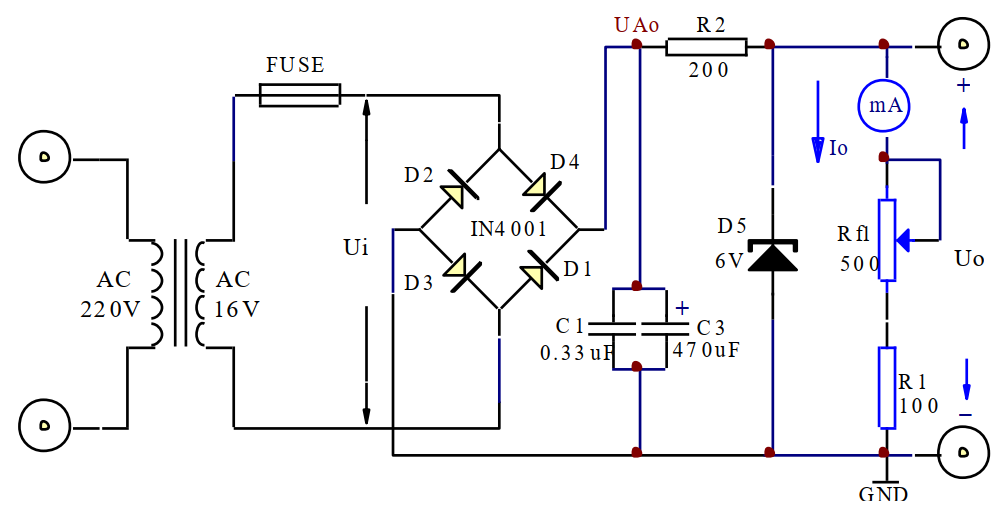
\includegraphics[width=0.4\textwidth]{稳压管电路图.png}
					\caption{稳压管并联稳压电路电路图}
					\label{fig:稳压管电路图}
				\end{figure}

				按照电路图\cref{fig:稳压管电路图}连接电路后,测量电路的输出效果,如图所示\cref{fig:稳压管效果1}:



				\begin{figure}[htbp]
					\centering
					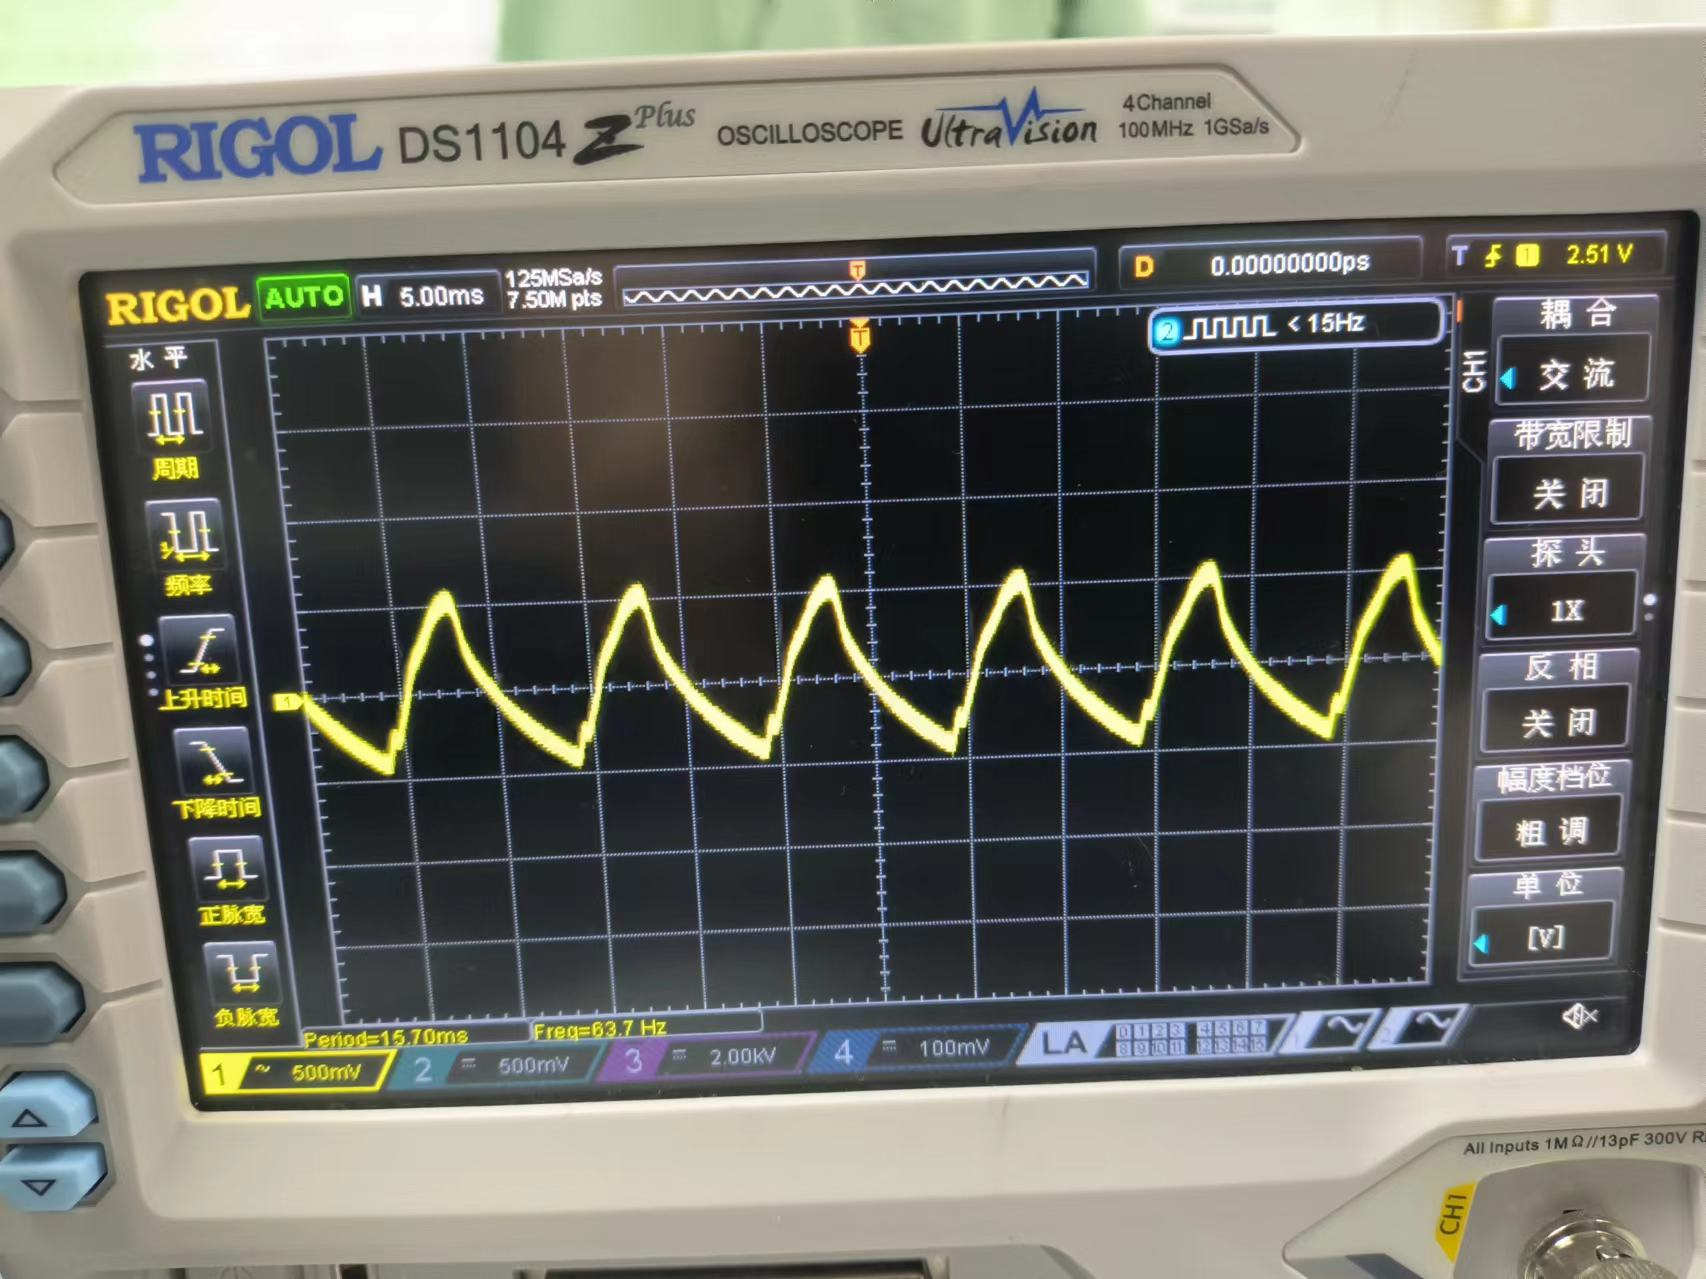
\includegraphics[width=0.4\textwidth]{稳压管效果1.jpg}
					\caption{稳压管并联稳压电路电路输出图像}
					\label{fig:稳压管效果1}
				\end{figure}



			\item 在桥式整流滤波电路中,搭建集成三端稳压器稳压电路,调整负载大小,观测并记录稳压电路的稳压效果;
			

				\begin{figure}[htbp]
					\centering
					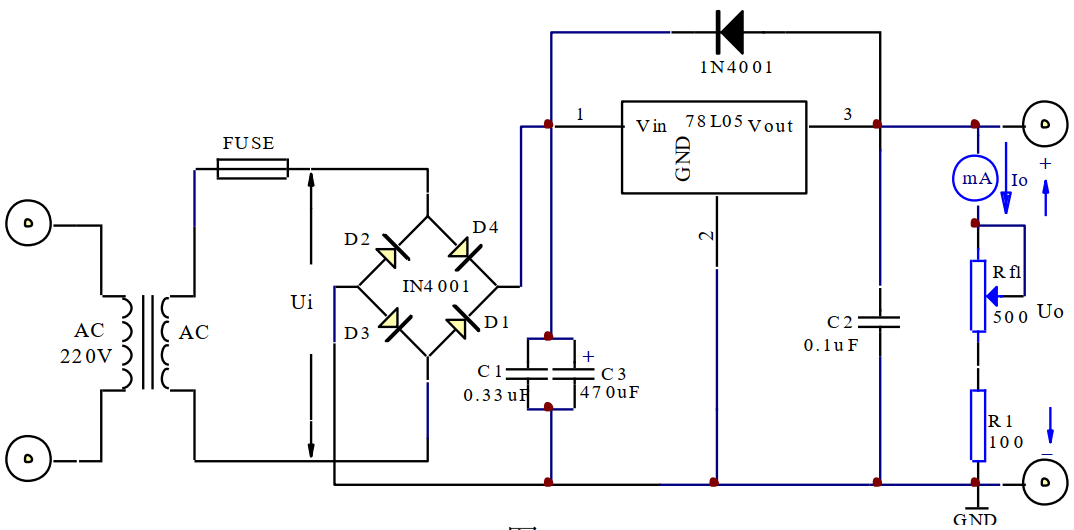
\includegraphics[width=0.4\textwidth]{三端集成稳压电路电路图.png}
					\caption{三端集成稳压电路电路图}
					\label{fig:三端集成稳压电路电路图}
				\end{figure}

				按照电路图\cref{fig:三端集成稳压电路电路图}连接电路后,测量电路的输出效果,如图所示\cref{fig:三端集成稳压电路效果1}:

				\begin{figure}[htbp]
					\centering
					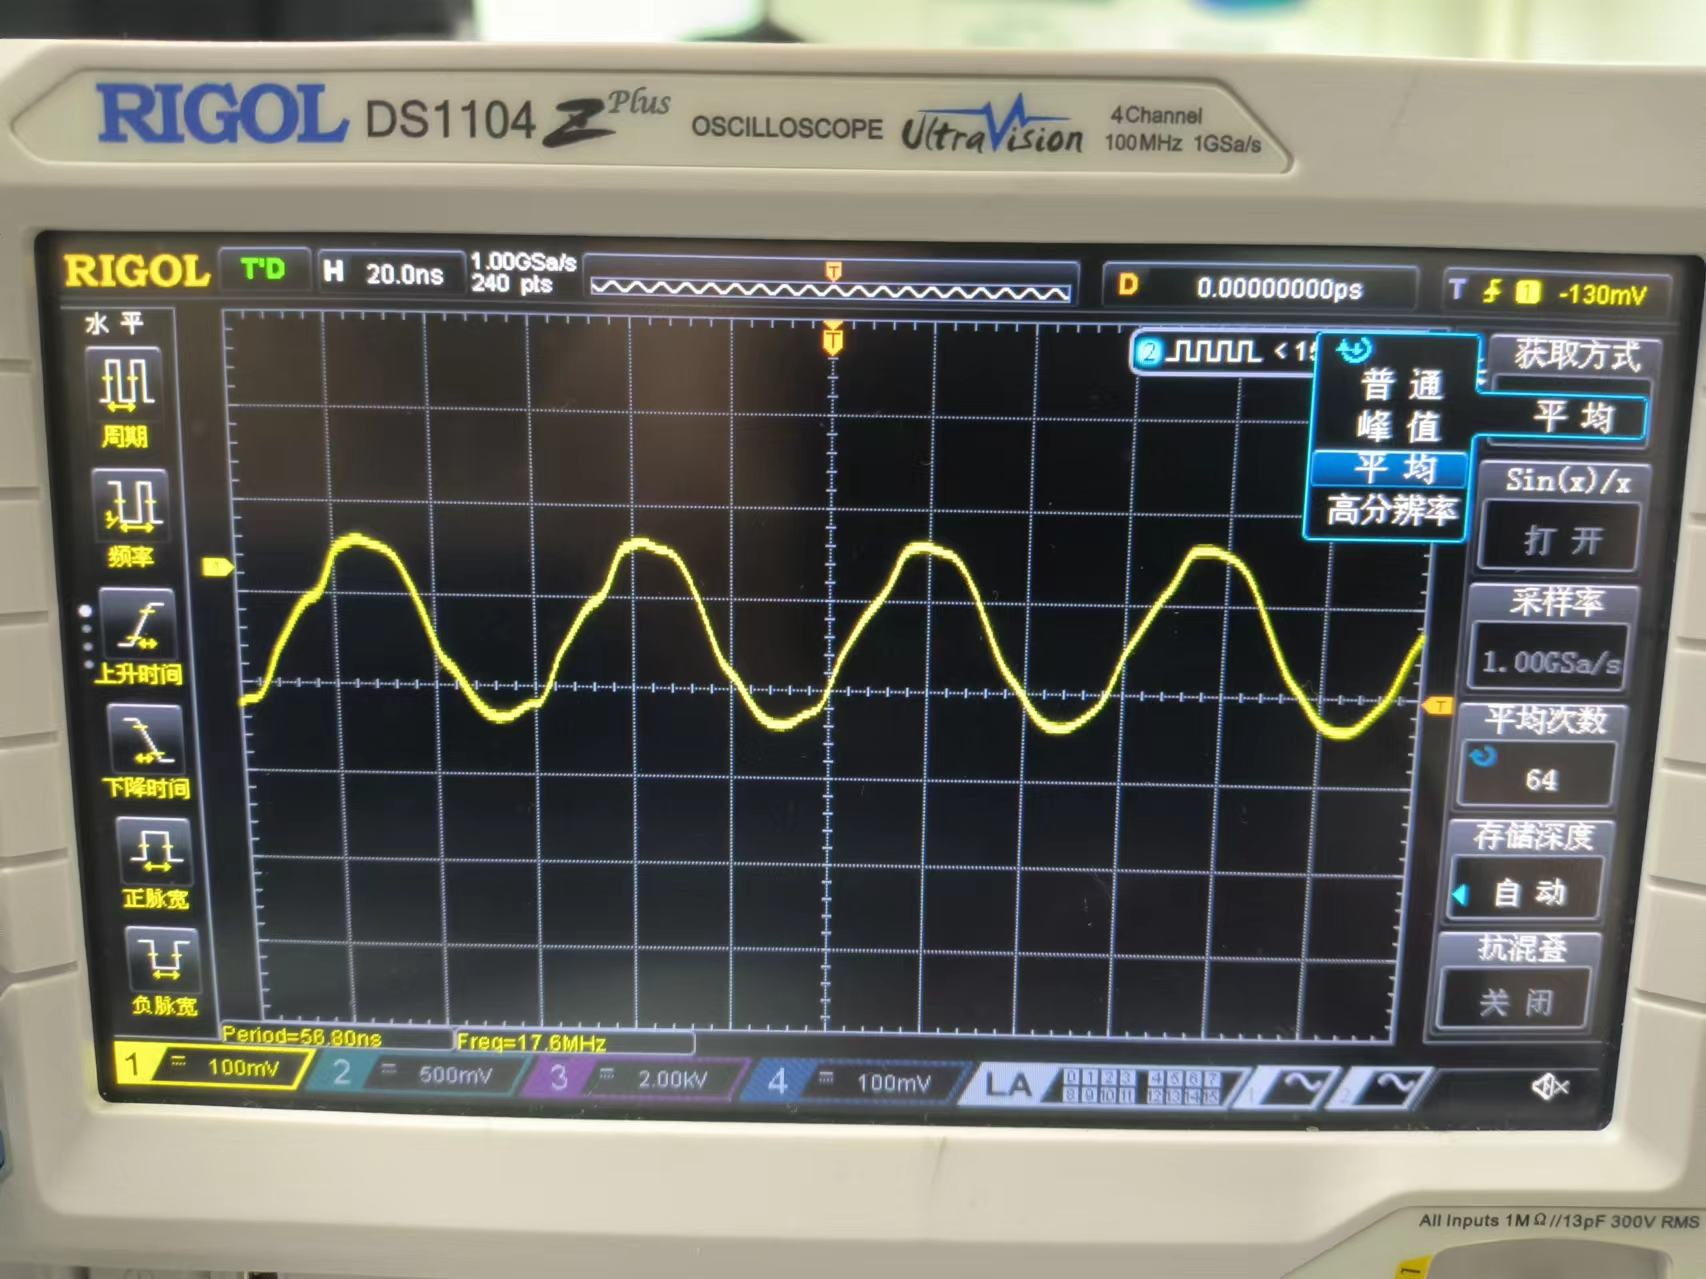
\includegraphics[width=0.4\textwidth]{三端集成稳压电路效果1.jpg}
					\caption{三端集成稳压电路输出图像}
					\label{fig:三端集成稳压电路效果1}
				\end{figure}











			\item 比较电路中稳压电路的输入输出效率;
			
				测量各个电路的输入、输出功率,并比较效率,结果如\cref{fig:稳压管并联稳压电路输入输出效率}、\cref{fig:三端集成稳压电路输入输出效率}所示:


				% \begin{table}
				% 	\centering
				% 	\begin{tblr}{
				% 		cells = {c},
				% 		cell{1}{1} = {c=3}{},
				% 		cell{1}{4} = {c=3}{},
				% 		vline{1-2,5,8} = {1}{},
				% 		vline{1,4,7-8} = {2-5}{},
				% 		hline{1-3,6} = {-}{},
				% 	}
				% 	输入端  &       &         & 输出端 &      &          & 效率       \\
				% 	$U_i$/V & $I_i$/mA & $P_{\text{in}}$ / W  & $R_L$/$\Omega$  & $U_o$/V   & $P_{\text{out}}$ / W       &          \\
				% 	2.3  & 121.6 & 0.27968 & 120 & 1.99 & 0.033001 & 0.117995 \\
				% 	2.3  & 121.5 & 0.27945 & 240 & 2.19 & 0.019984 & 0.071511 \\
				% 	2.3  & 121.6 & 0.27968 & 360 & 2.27 & 0.014314 & 0.051179 
				% 	\end{tblr}
				% 	\caption{稳压管并联稳压电路输入输出效率}
				% 	\label{fig:稳压管并联稳压电路输入输出效率}
				% \end{table}

				\begin{table}
					\centering
					\begin{tblr}{
					  cells = {c},
					  cell{1}{1} = {r=2}{},
					  cell{1}{2} = {c=3}{},
					  cell{1}{5} = {c=2}{},
					  cell{1}{7} = {r=2}{},
					  vline{1-3,5,7,8} = {1}{},
					  vline{1,2,5,7,8} = {2}{},
					  vline{1-2,5,7,8} = {3-5}{},
					  hline{1,3,6} = {-}{},
					  hline{2} = {2-6}{},
					}
					负载电阻$R_L/\Omega$ & 输入端  &       &         & 输出端  &          & 效率$\eta = \frac{P_{o}}{P_{i}}$      \\
						 & $U_i/V$ & $I_i/mA$ & $P_{i}/W$       & $U_o/V$   & $P_{o}/W$       &         \\
					120  & 15.32 & 107.4   & 1.645368  & 4.08 & 0.13872 & 8.43\% \\
					240  & 15.33 & 107.84  & 1.6531872 & 4.11 & 0.07038375 & 4.26\% \\
					360  & 15.32 & 107.55  & 1.647666  & 4.13 & 0.047380278 & 2.88\% 
					\end{tblr}
					\caption{稳压管并联稳压电路输入输出效率}
					\label{fig:稳压管并联稳压电路输入输出效率}
				\end{table}
			


				\begin{table}
					\centering
					\begin{tblr}{
					  cells = {c},
					  cell{1}{1} = {r=2}{},
					  cell{1}{2} = {c=3}{},
					  cell{1}{5} = {c=2}{},
					  cell{1}{7} = {r=2}{},
					  vline{1-3,5,7,8} = {1}{},
					  vline{1,2,5,7,8} = {2}{},
					  vline{1-2,5,7,8} = {3-5}{},
					  hline{1,3,6} = {-}{},
					  hline{2} = {2-6}{},
					}
					负载电阻$R_L/\Omega$ & 输入端  &       &         & 输出端  &          & 效率$\eta = \frac{P_{o}}{P_{i}}$      \\
						 & $U_i/V$ & $I_i/mA$ & $P_{i}/W$       & $U_o/V$   & $P_{o}/W$       &         \\
					120  & 14.2 & 102   & 1.4484  & 11.6 & 1.121333 & 77.42\% \\
					240  & 16.6 & 55.3  & 0.91798 & 12.2 & 0.620167 & 67.56\% \\
					360  & 17.4 & 38.8  & 0.67512 & 12.1 & 0.406694 & 60.24\% 
					\end{tblr}
					\caption{三端集成稳压电路输入输出效率}
					\label{fig:三端集成稳压电路输入输出效率}
				\end{table}






		\end{enumerate}
	




	%
	% \subsubsection{实验结果展示}
	
	
	% ---
	



	% 原始数据
	\clearpage
	\subsection{原始数据记录}
	实验记录本上的原始数据见\cref{fig:figO1}与\cref{fig:figO2}(签字)。
	
	% \begin{figure}[htbp]
	% 	\centering
	% 	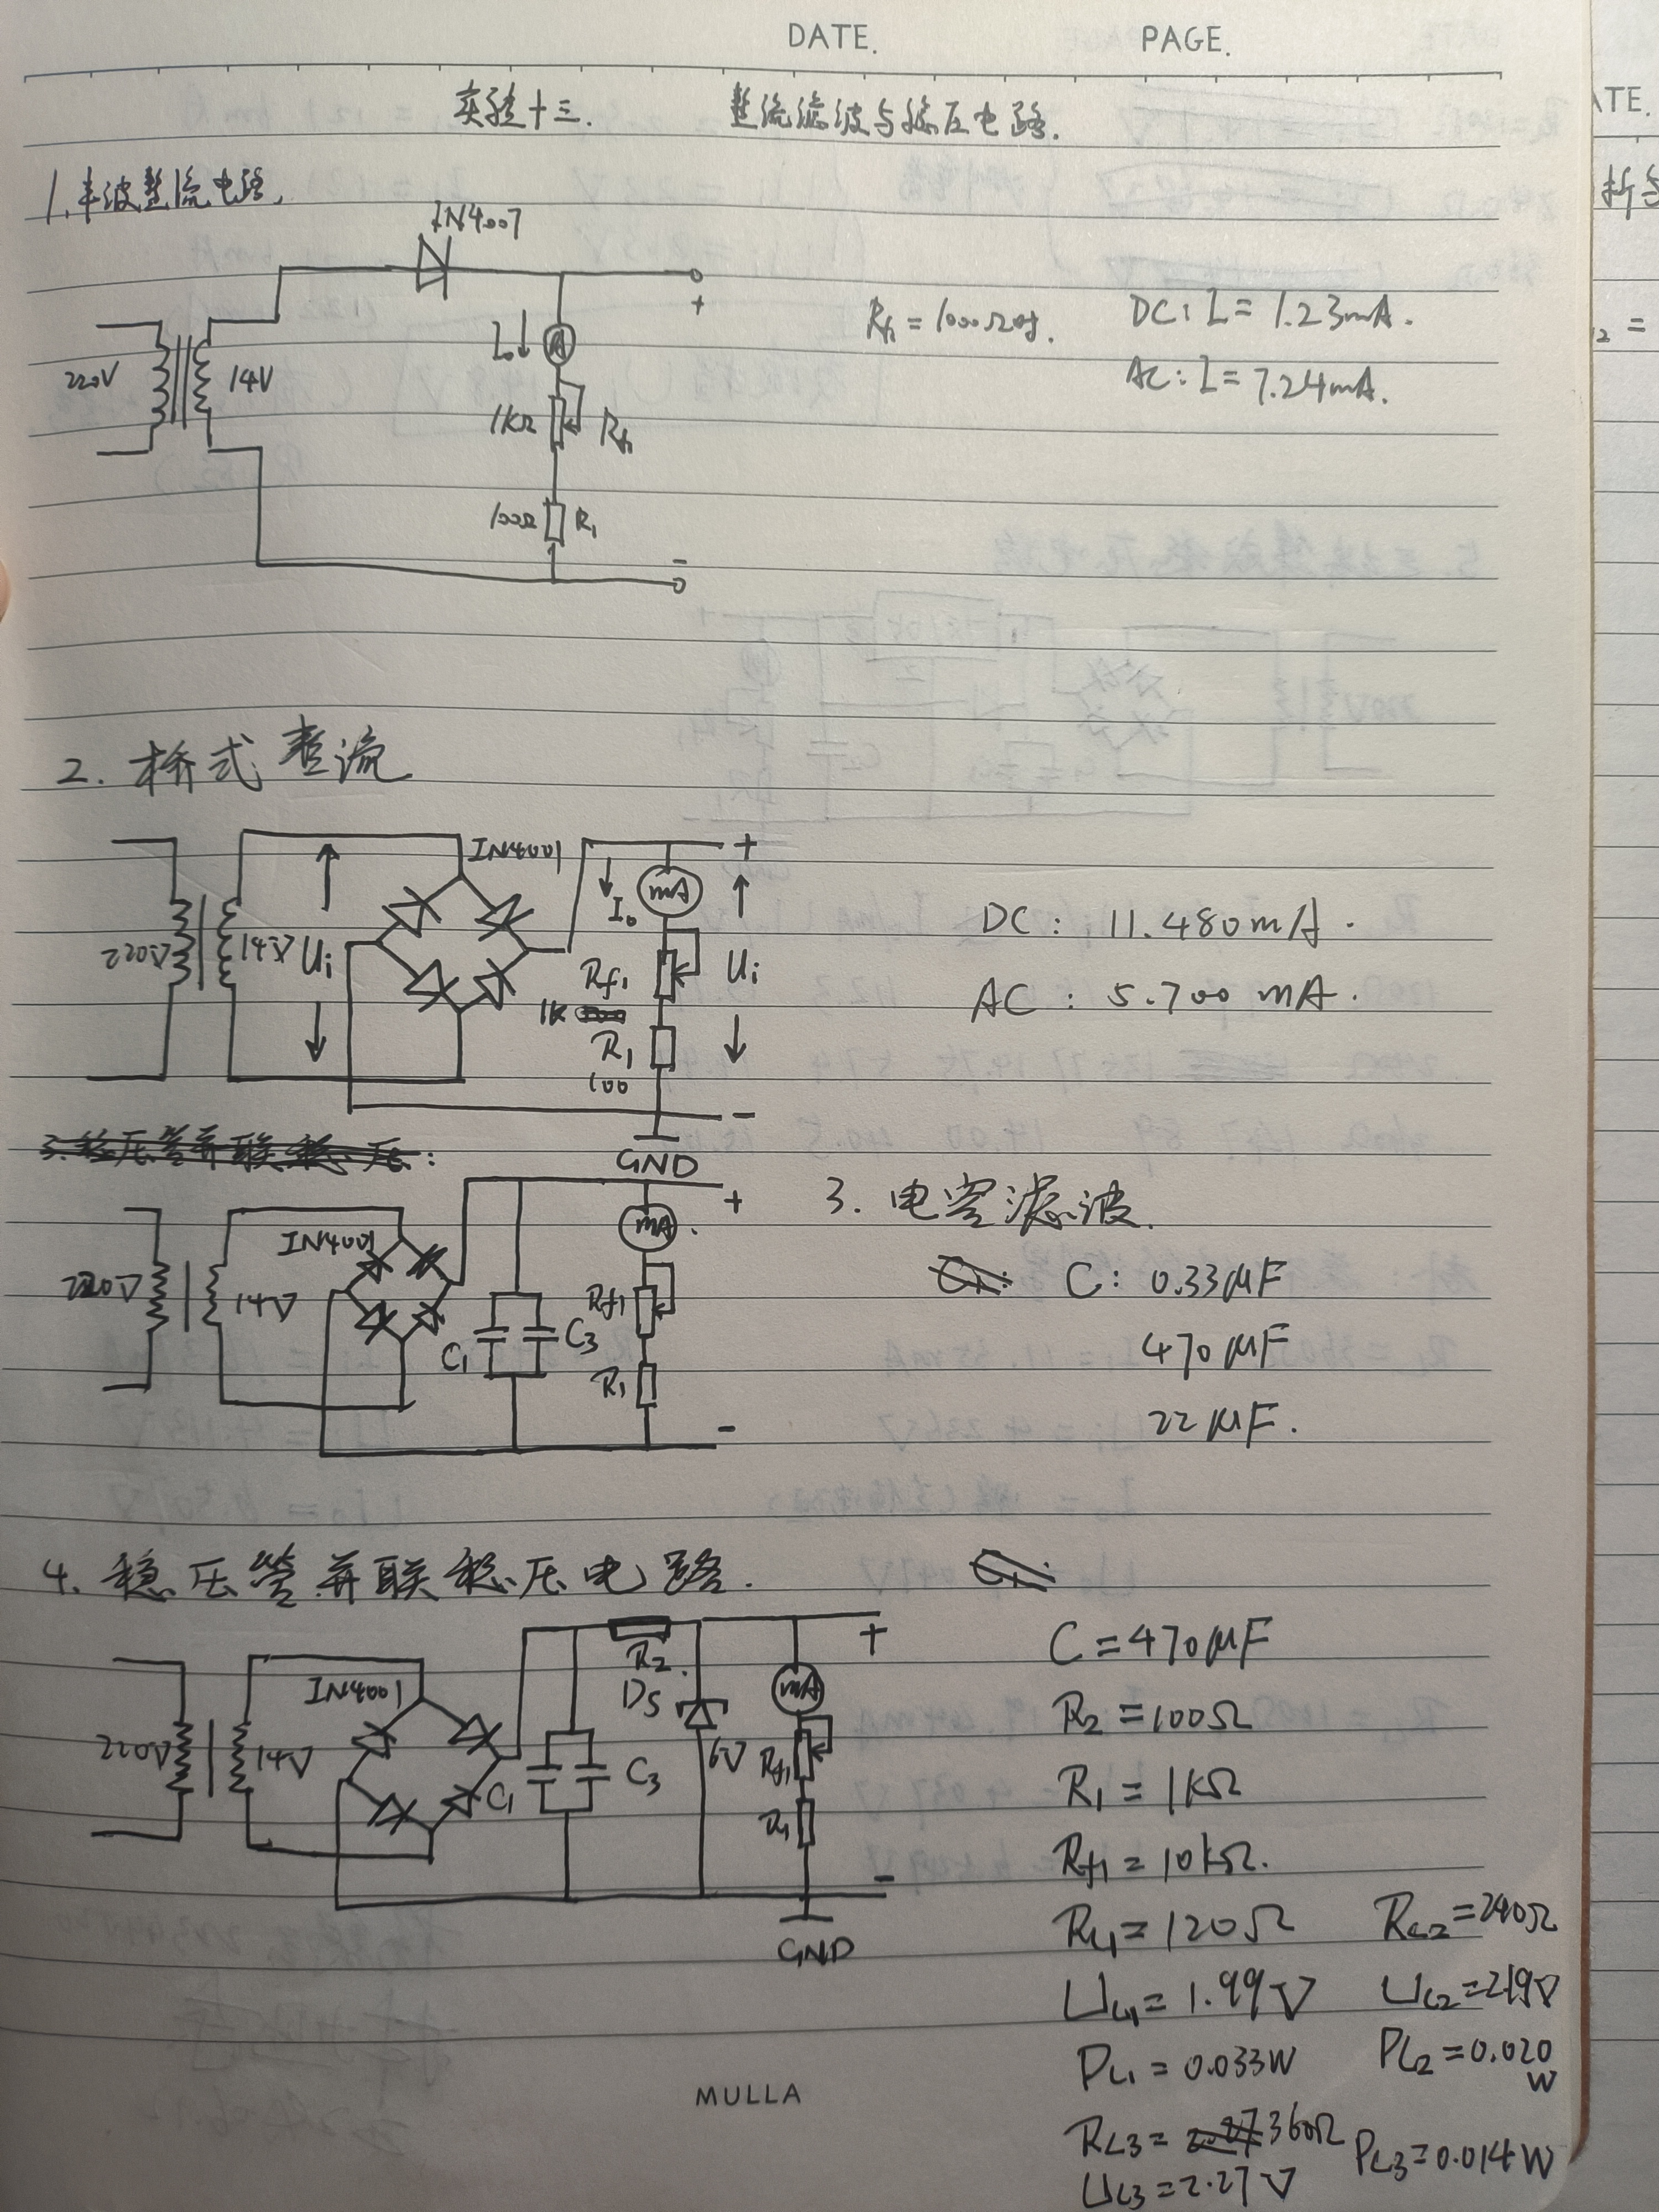
\includegraphics[width=0.38\textwidth]{ET1_13GraO1.jpg}
	% 	\caption{原始数据记录1}
	% 	\label{fig:figO1}
	% \end{figure}
		
	% \begin{figure}[htbp]
	% 	\centering
	% 	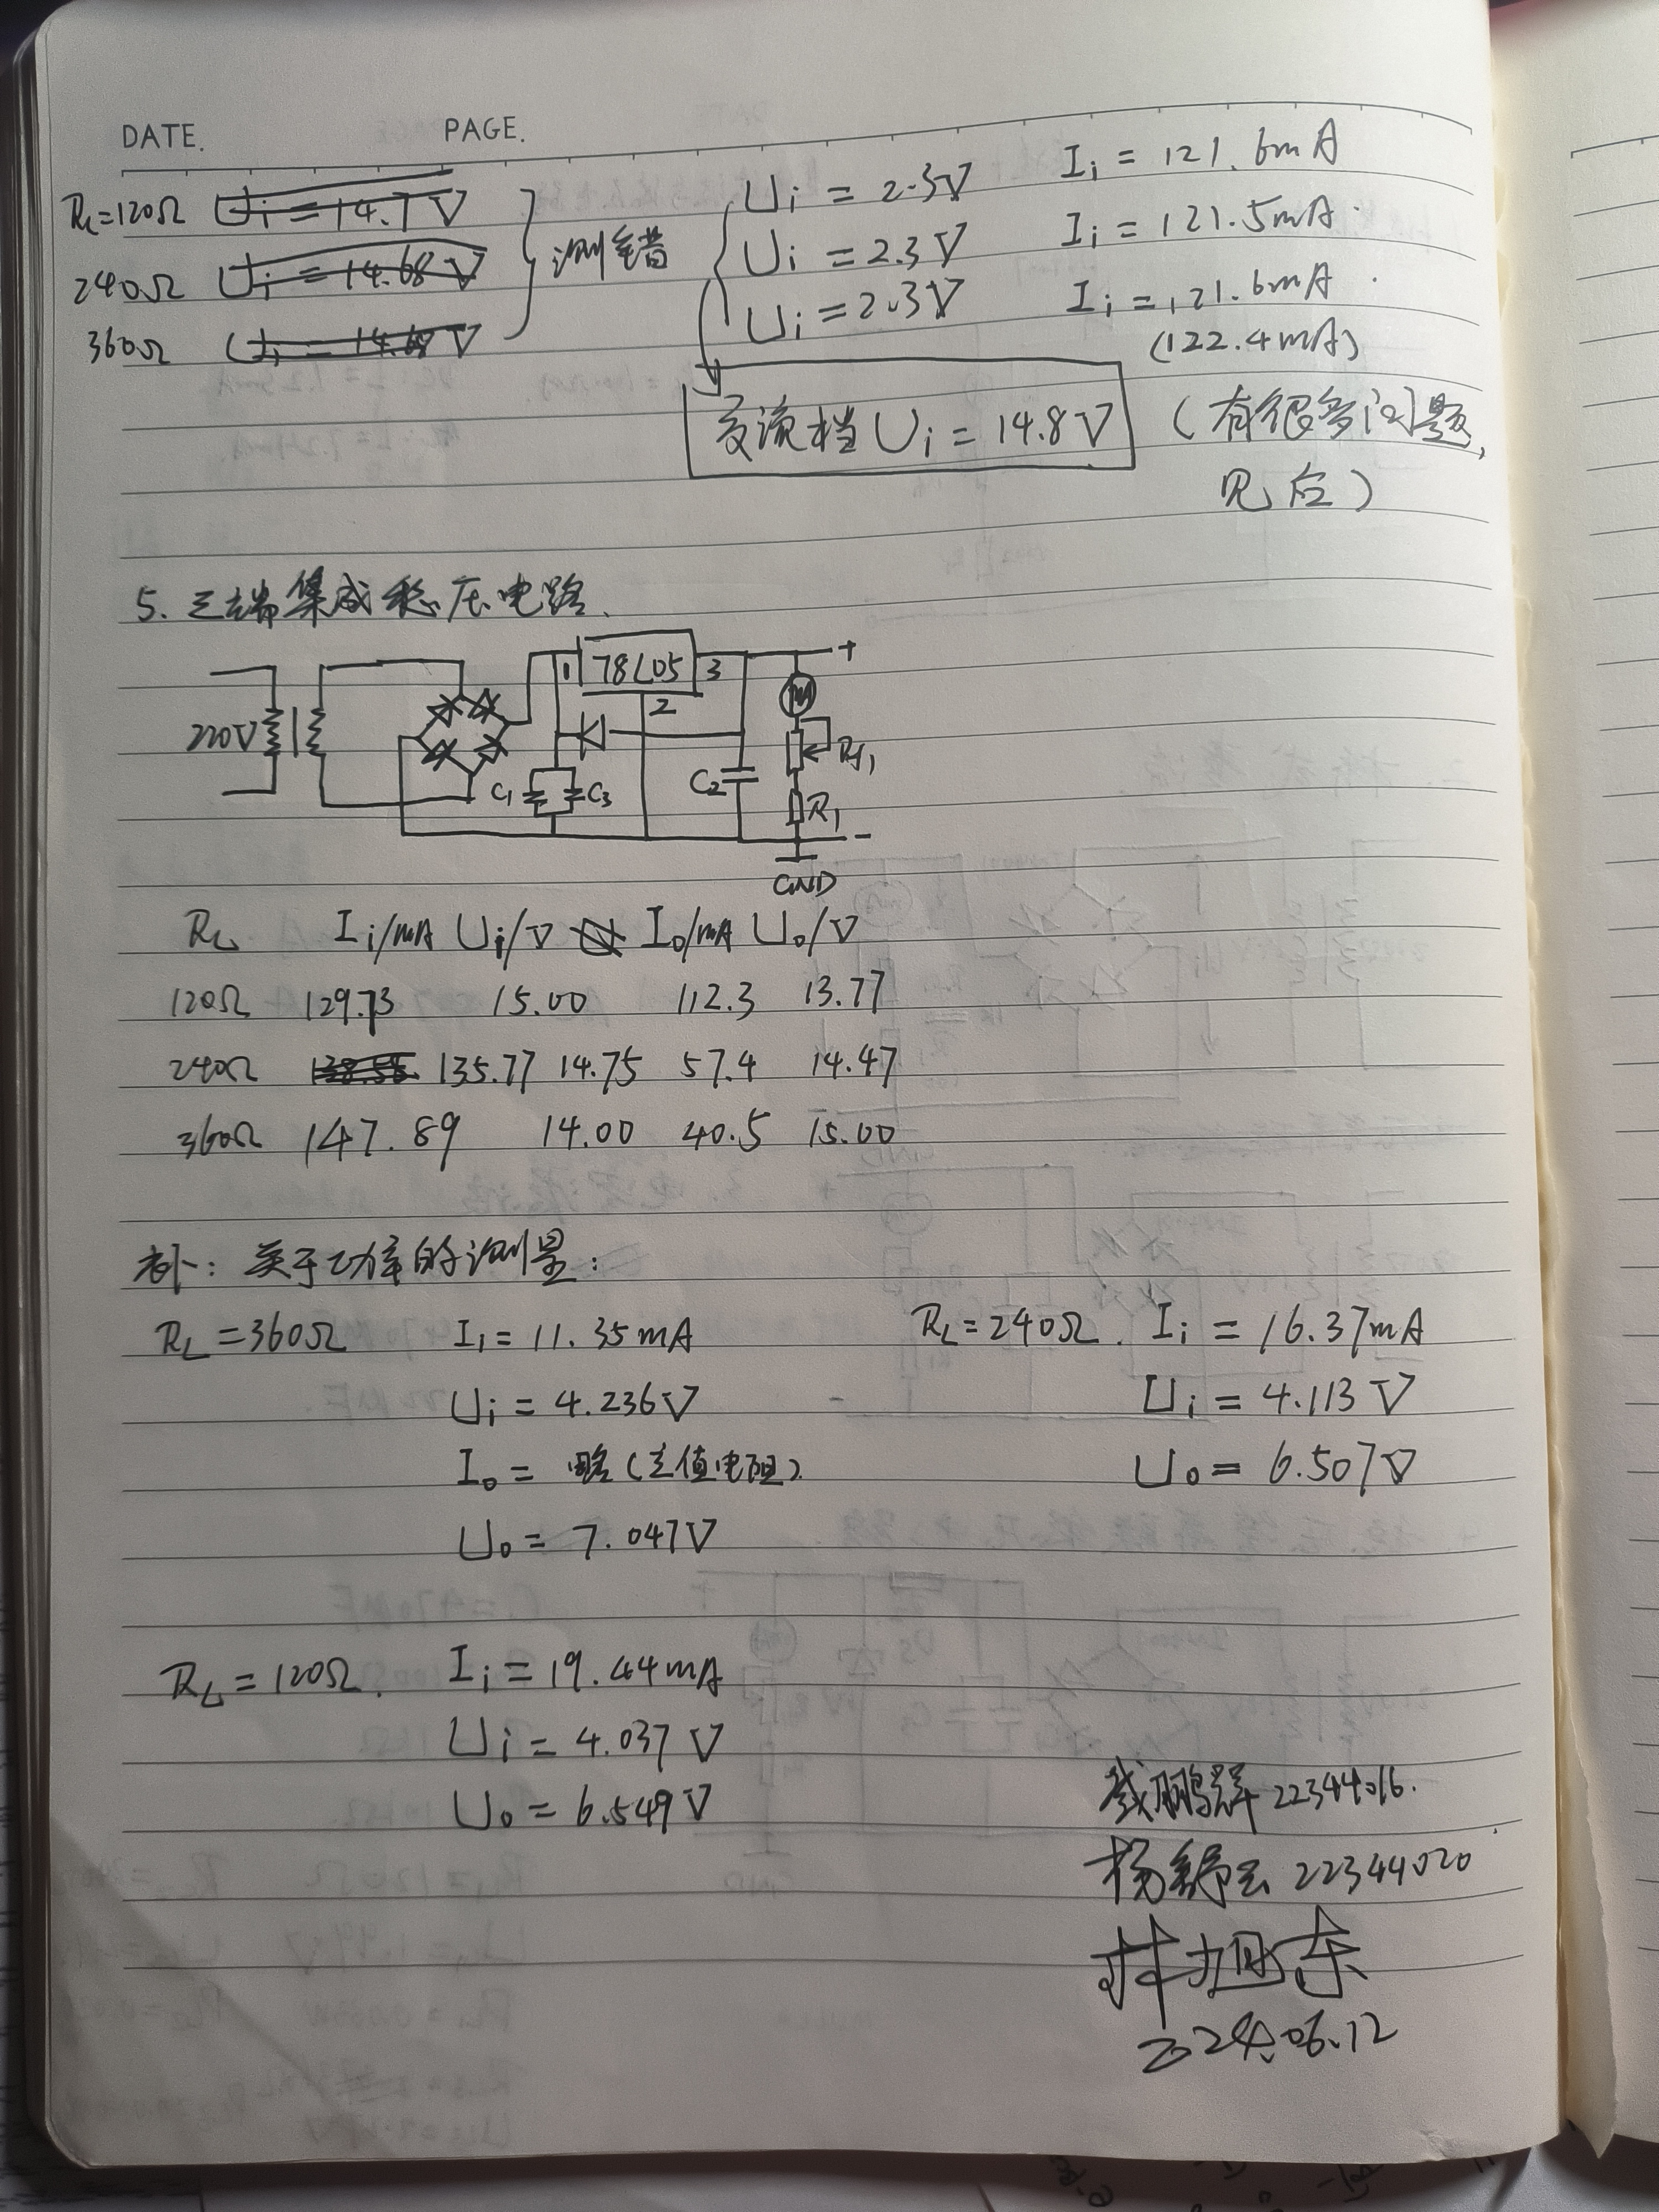
\includegraphics[width=0.38\textwidth]{ET1_13GraO2.jpg}
	% 	\caption{原始数据记录2}
	% 	\label{fig:figO2}
	% \end{figure}

	\begin{figure}[htbp]
		\centering
		\subfloat[原始数据1]
		{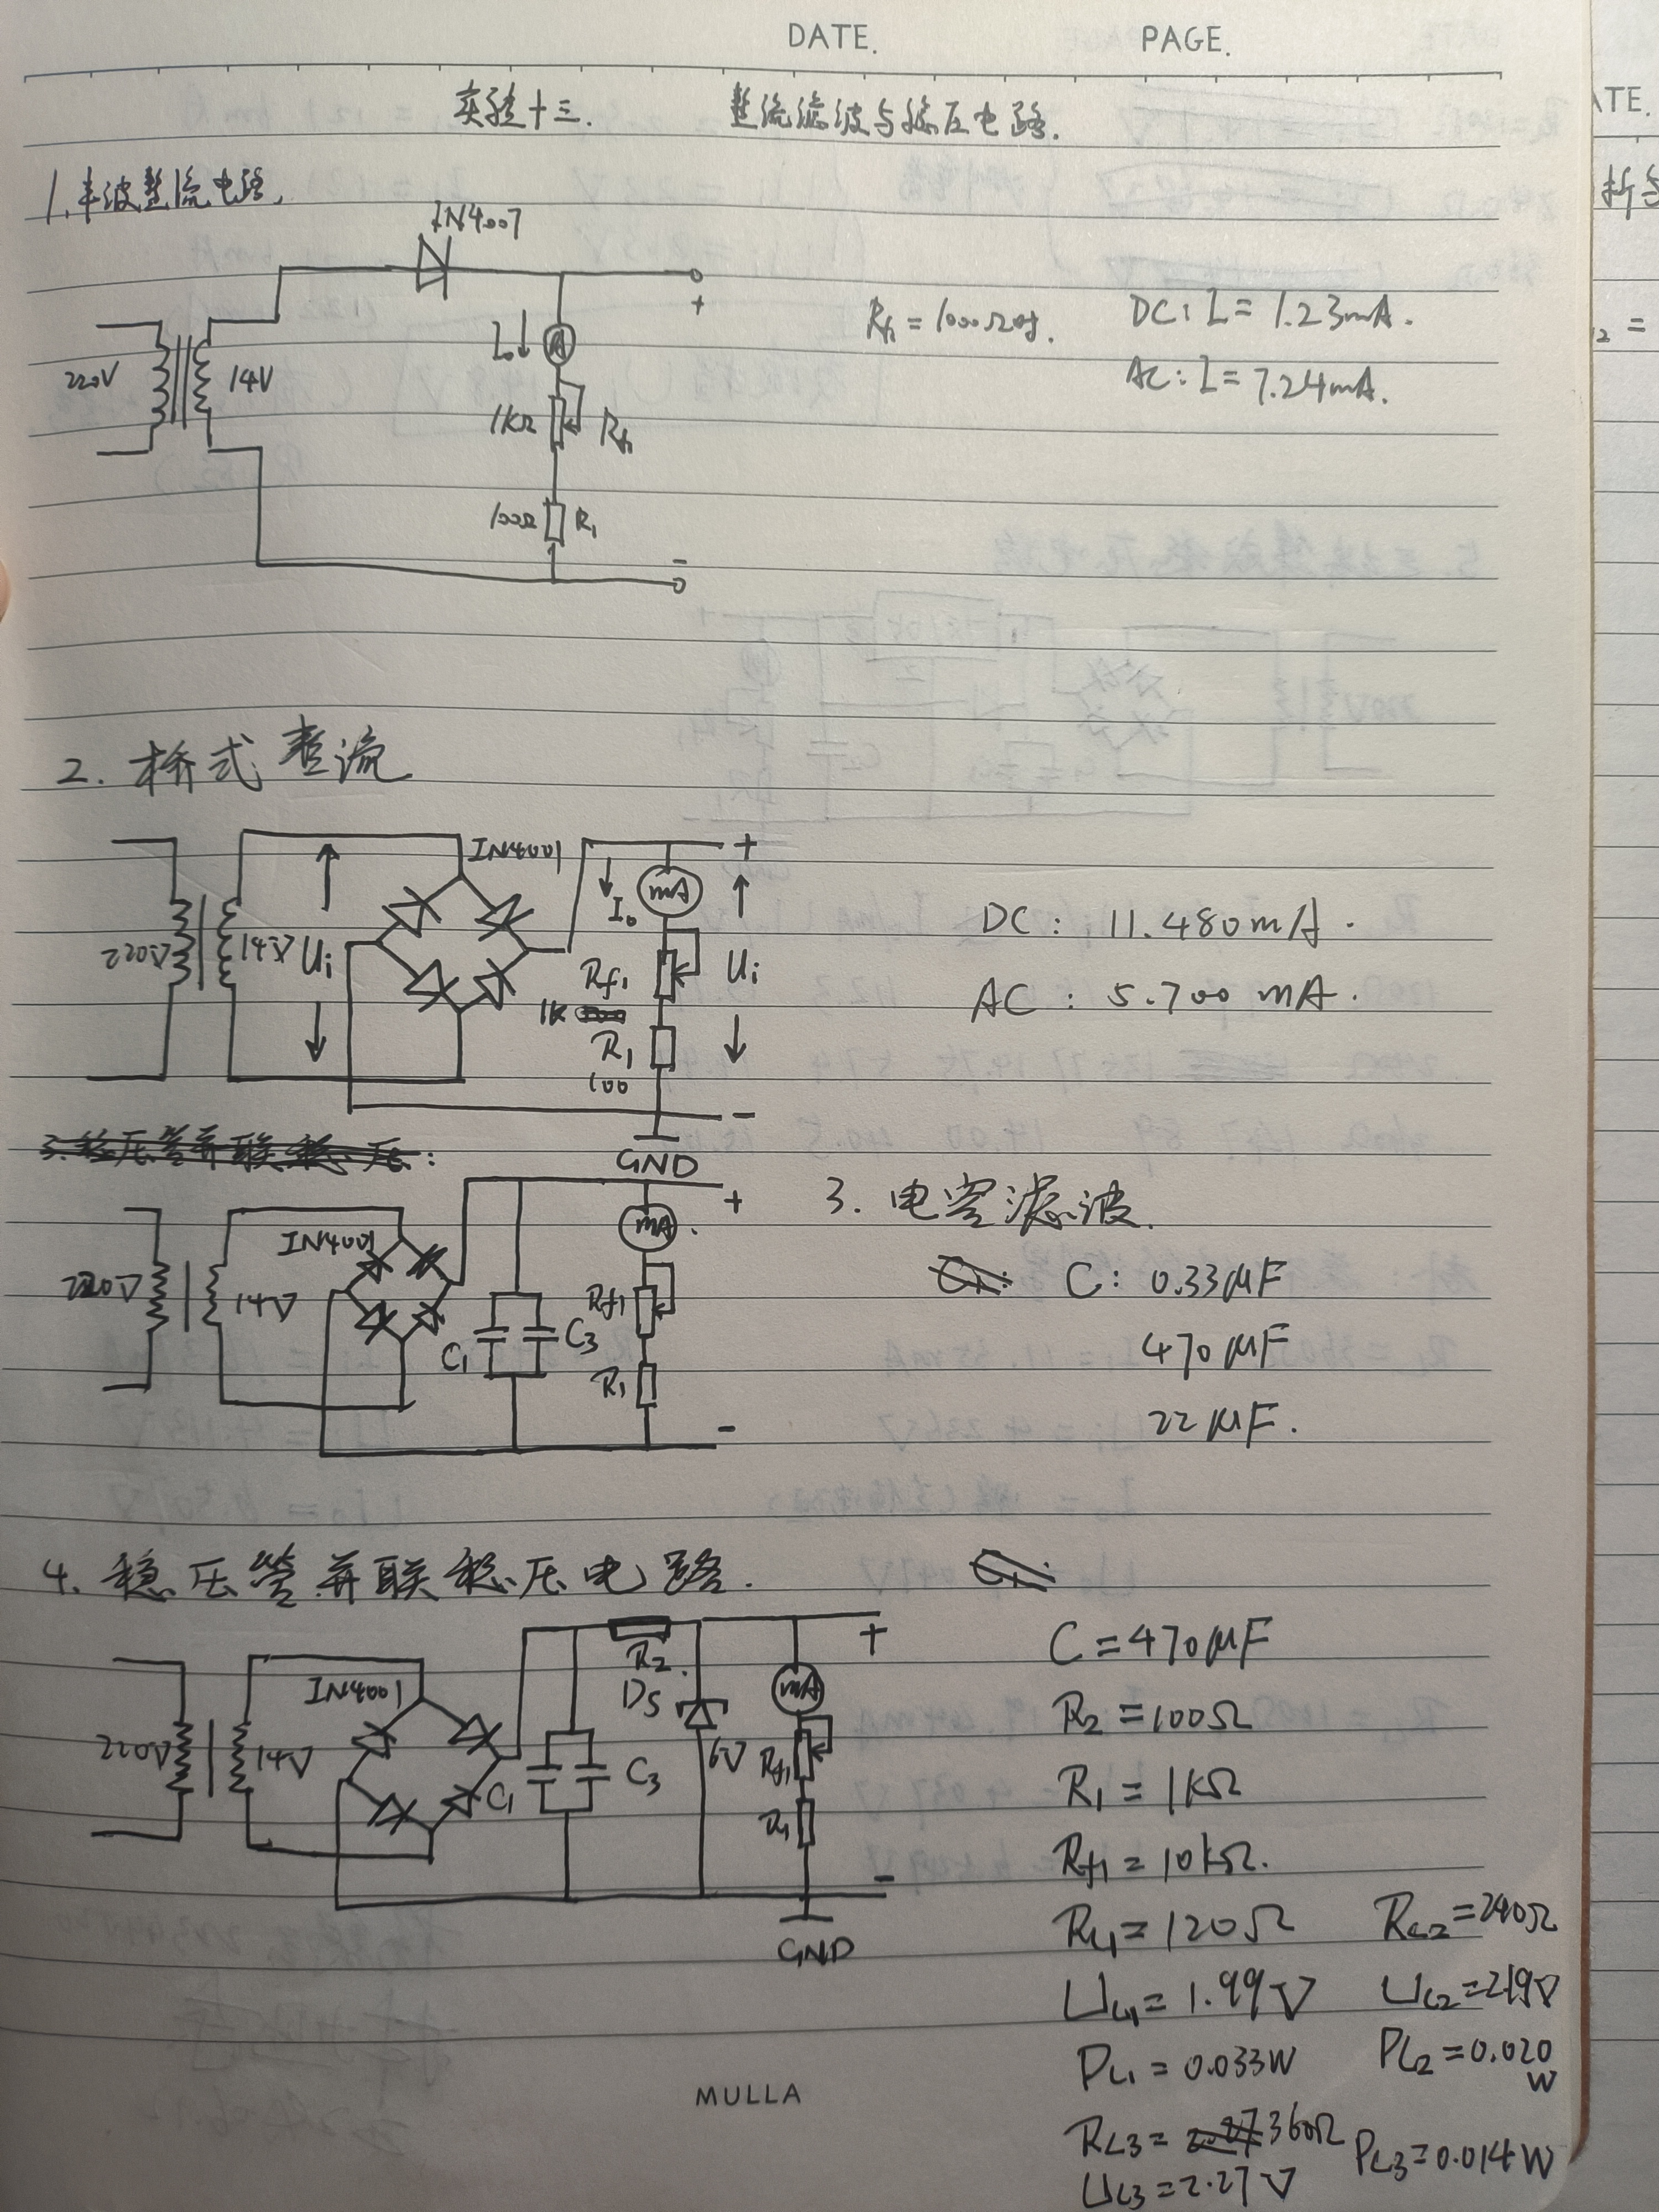
\includegraphics[width=0.45\textwidth]{ET1_13GraO1.jpg}\label{fig:figO1}}
		\quad
		\subfloat[原始数据2]
		{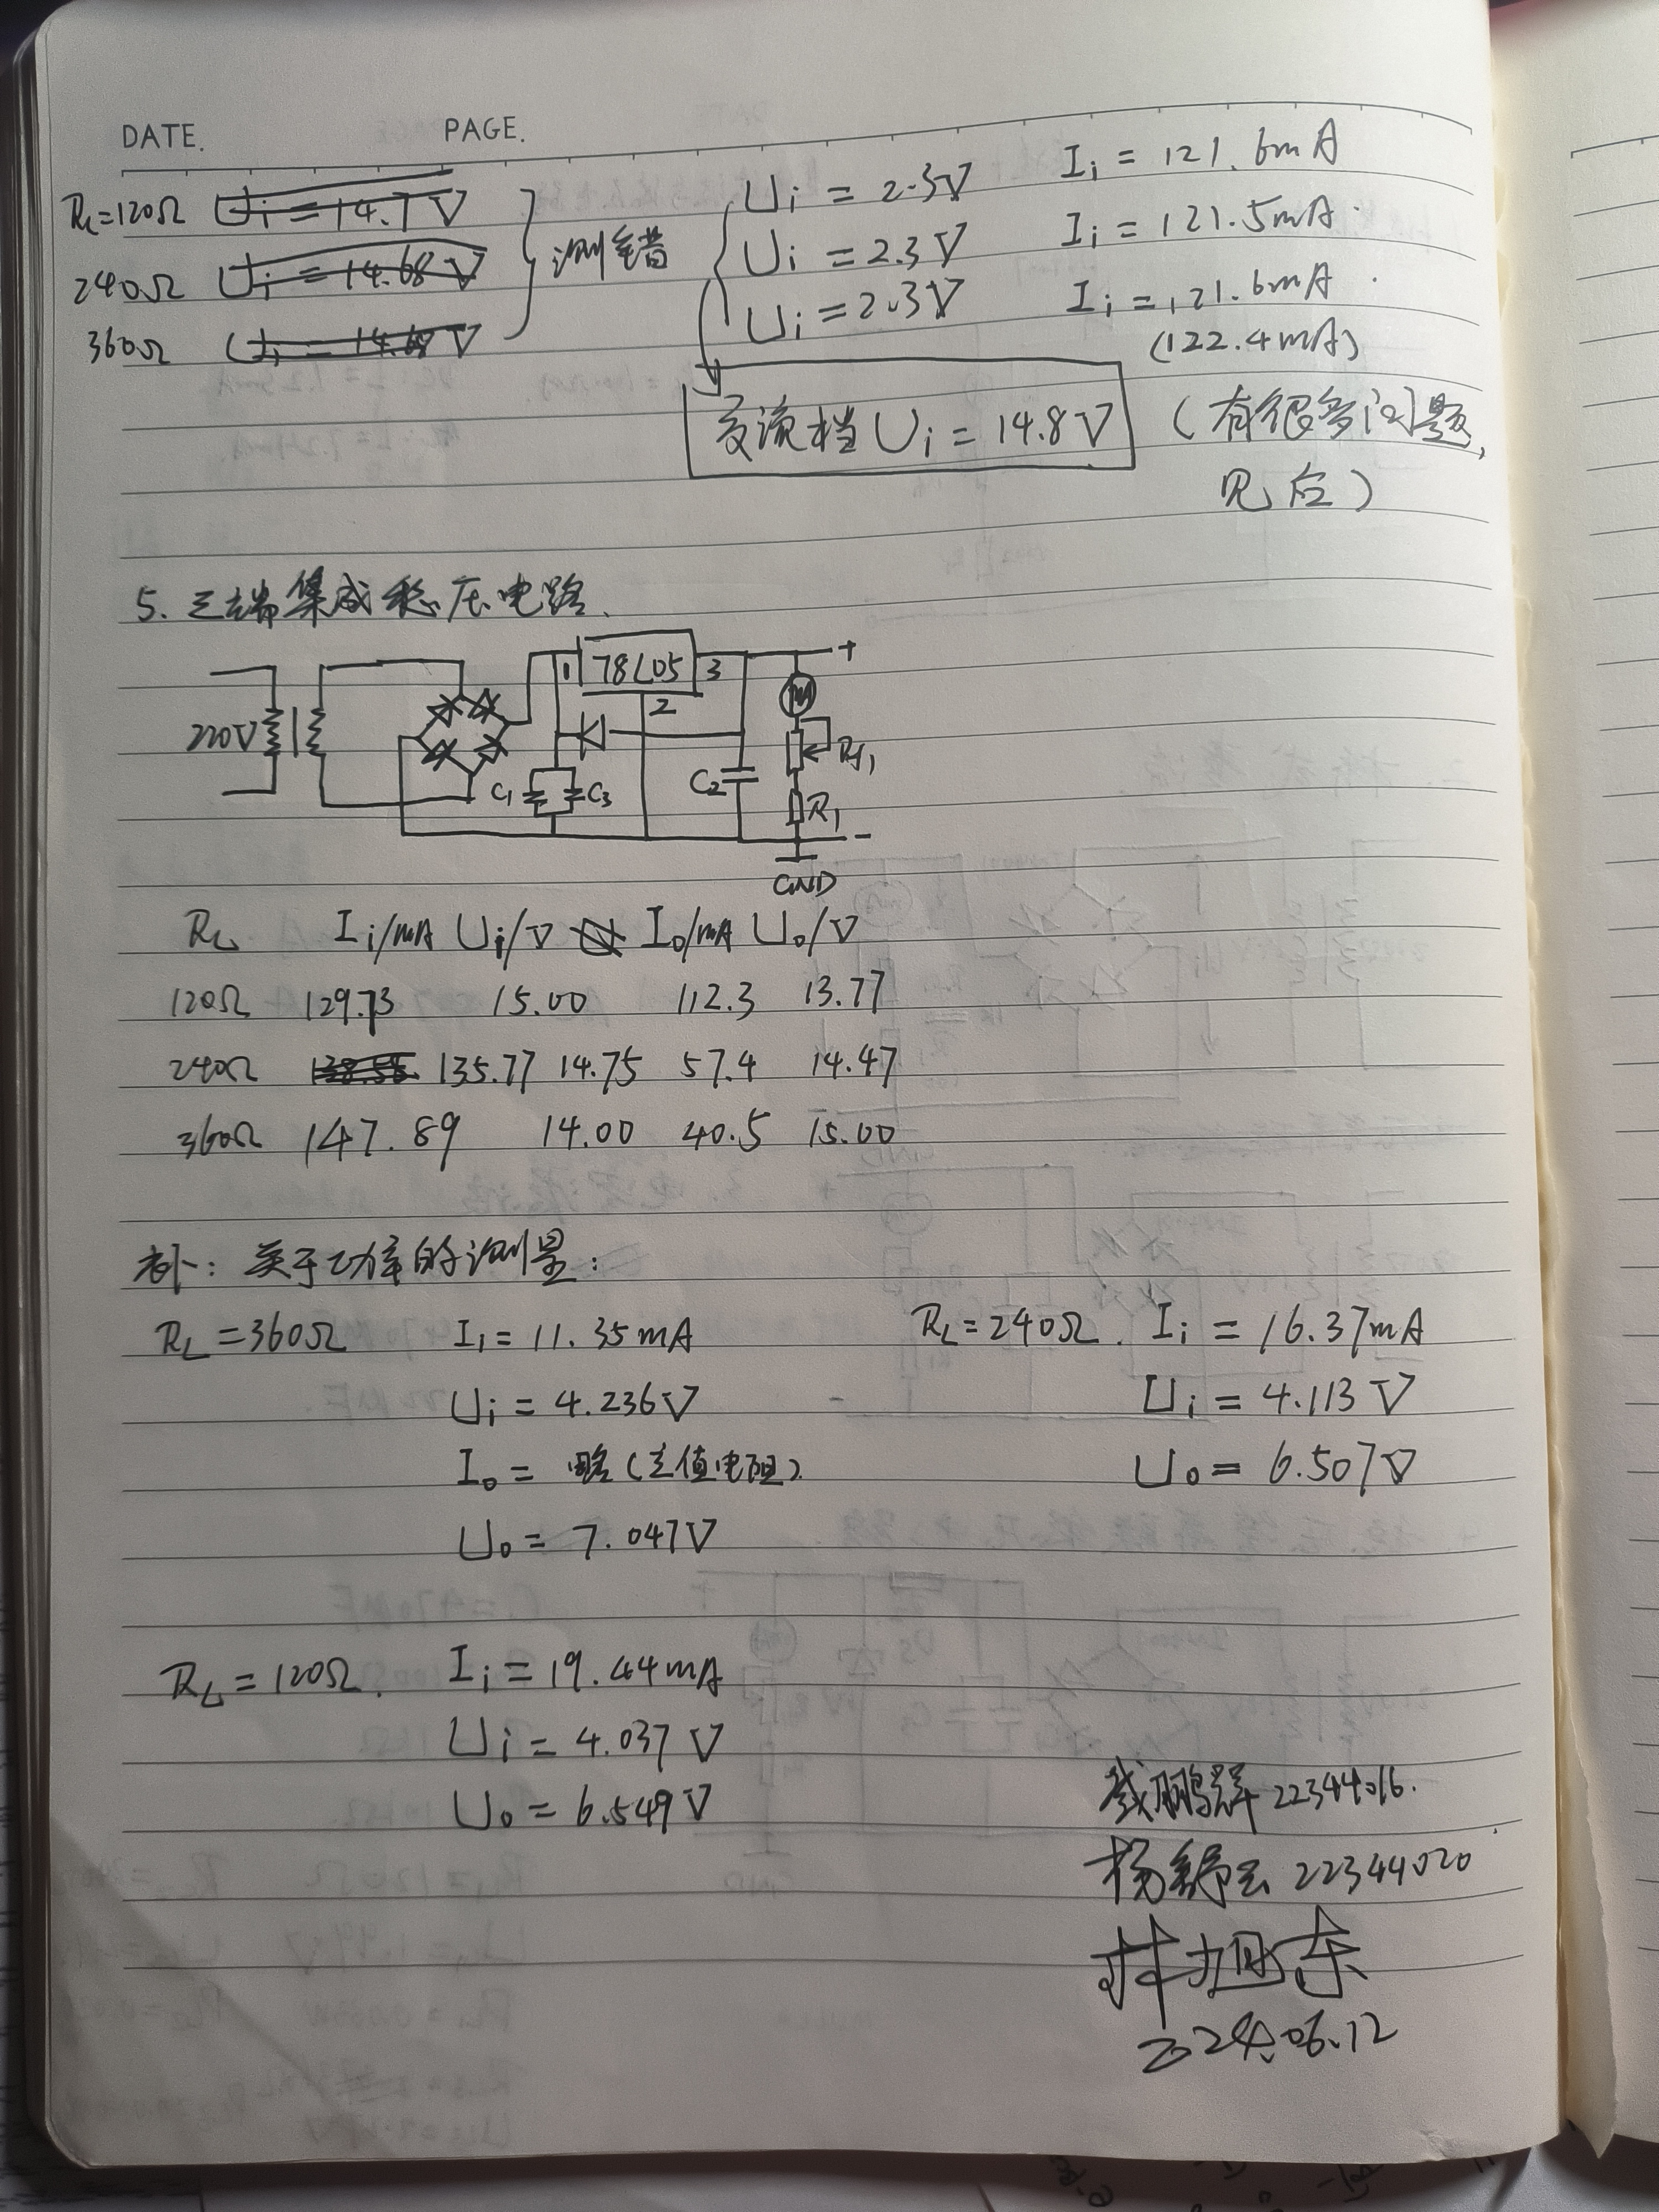
\includegraphics[width=0.45\textwidth]{ET1_13GraO2.jpg}\label{fig:figO2}}
		\quad

		% \caption{原始数据记录}
		\label{fig:data}
	\end{figure}
	
	%实验台桌面整理见%\textbf{附件}部分(\cref{})。
	
	%其它原始数据见%\cref{}。
	% ---
	
	% 问题记录
	%\subsection{实验过程遇到问题及解决办法}
	
	% ---
	
	
	
	% 分析与讨论	
	\clearpage
	
	% 顶栏
	\begin{table}
		\renewcommand\arraystretch{1.7}
		\begin{tabularx}{\textwidth}{|X|X|X|X|}
			\hline
			专业:& 物理学 &年级:& 2022级\\
			\hline
			姓名: & 戴鹏辉、杨舒云 & 学号:& 22344016、22344020\\
			\hline
			日期:& 2024/6/12 & 评分: &\\
			\hline
		\end{tabularx}
	\end{table}
	% ---
	
	% 小标题
	\section{ET1-13 整流滤波与稳压电路 \quad\heiti 分析与讨论}
	% ---
	
	% 数据处理
	\subsection{实验数据分析}
	
		\begin{enumerate}
			\item 搭建半波整流电路,用示波器观测和记录输出波形;
			
				如\cref{fig:半波整流}所示,交流电经过半波整流电路后,一个周期内一半时间有正弦波,一半时间为0,且输出信号周期为20ms(即50Hz),与市电一致。






			\item 搭建桥式整流电路, 用示波器观测和记录输出波形;
			

				如\cref{fig:全波整流}所示,交流电经过桥式整流电路后,一个周期内没有输出为零的时刻。且输出信号周期为10ms(即100Hz),为市电的两倍,因为此时负半轴的波被翻至正半轴,原本的一个周期变为两个周期,频率便翻倍了。



				% 下面对半波整流和桥式全波整流做比较:

				% \begin{itemize}
				% 	\item \textbf{半波整流}:
				% 	\begin{itemize}
				% 		\item \textbf{电路结构简单}:半波整流电路只需要一个二极管,电路结构非常简单。
				% 		\item \textbf{效率低}:由于只有交流电的一个半周期被整流,另一半周期被浪费,整流效率较低。
				% 		\item \textbf{输出波形}:输出波形为单向的脉动直流,含有大量的纹波,平滑度较差。
				% 		\item \textbf{平均输出电压低}:由于只有一个半周期被整流,平均输出电压大约是输入电压峰值的 $\frac{1}{\pi}$ 倍。
				% 		\item \textbf{应用场合}:由于其效率低和输出电压不稳定,半波整流通常只用于对电源质量要求不高的简单电路中。
				% 	\end{itemize}
				
				% 	\item \textbf{桥式全波整流}:
				% 	\begin{itemize}
				% 		\item \textbf{电路结构复杂}:桥式全波整流电路需要四个二极管,电路结构相对复杂。
				% 		\item \textbf{效率高}:利用交流电的两个半周期进行整流,整流效率较高。
				% 		\item \textbf{输出波形}:输出波形为双向的脉动直流,相对于半波整流,纹波频率是输入交流电频率的两倍,较为平滑。
				% 		\item \textbf{平均输出电压高}:由于两个半周期都被整流,平均输出电压大约是输入电压峰值的 $\frac{2}{\pi}$ 倍。
				% 		\item \textbf{应用场合}:由于其效率高和输出电压相对稳定,桥式全波整流广泛应用于各种需要稳定直流电源的电子设备中。
				% 	\end{itemize}
				% \end{itemize}
				
				% \begin{table}[h]
				% \centering
				% \begin{tabular}{|c|c|c|}
				% \hline
				% \textbf{特点}     & \textbf{半波整流} & \textbf{桥式全波整流} \\ \hline
				% 电路结构 & 简单             & 复杂             \\ \hline
				% 效率     & 低               & 高               \\ \hline
				% 输出波形 & 单向脉动直流     & 双向脉动直流     \\ \hline
				% 平均输出电压 & 低               & 高               \\ \hline
				% 应用场合 & 简单电路         & 各种需要稳定直流电源的设备 \\ \hline
				% \end{tabular}
				% \caption{半波整流与桥式全波整流的比较}
				% \end{table}
				
				% 简而言之,半波整流和桥式全波整流各有其优缺点。半波整流电路简单但效率低,适用于对电源质量要求不高的场合;桥式全波整流效率高但电路较复杂,适用于需要稳定直流电源的电子设备。
				



			\item 加入滤波电容
			
				在刚刚全波桥式整流电路的基础上,加入滤波电容后,得到的结果如\cref{fig:全波整流+滤波电容1}、\cref{fig:全波整流+滤波电容2}所示:

				单独并联0.33$\mu F$的电容时,得到的结果如\cref{fig:全波整流+滤波电容1},还是可以看到较明显的波纹;
				
				并联470$\mu F$的电容时,得到的结果如\cref{fig:全波整流+滤波电容2}所示,滤波效果较好,基本滤去了波纹,输出波形平滑。\\

				
				
				在桥式全波整流电路中并联滤波电容,选择不同大小的电容会对输出波形产生显著影响。具体而言,滤波电容的大小直接影响输出电压的平滑程度和纹波电压的幅度。

				\begin{itemize}
					\item 小电容:

						\begin{itemize}
							\item \textbf{滤波效果较差}:小电容的充放电时间常数较小,无法充分平滑整流后的波形。
							\item \textbf{纹波电压较大}:由于小电容不能有效地储存和释放电能,输出电压中的交流成分(纹波)仍然比较大,输出波形较不平滑。
							\item \textbf{输出电压变化较大}:小电容导致输出电压的波动较大,接近原始整流后的脉动直流电压。
						\end{itemize}

					\item 大电容:
					
						\begin{itemize}
							\item \textbf{滤波效果较好}:大电容的充放电时间常数较大,能够更有效地平滑整流后的波形。
							\item \textbf{纹波电压较小}:大电容能够储存更多的电能并在负载需要时释放,显著减少输出电压中的交流成分,使输出电压更加平稳。
							\item \textbf{输出电压更接近理想的直流电压}:大电容能更好地保持输出电压的恒定,提供更加稳定的直流输出。
						\end{itemize}
						
				\end{itemize}

				

				
				以下是选择不同大小电容对输出波形的具体影响:
				
				\begin{itemize}
					\item \textbf{无滤波电容}:
					\begin{itemize}
						\item 输出电压为脉动的全波整流波形,具有较大的纹波电压,频率为输入交流电的两倍。
					\end{itemize}
					\item \textbf{小滤波电容}:
					\begin{itemize}
						\item 输出电压波形略有平滑,但仍具有明显的纹波电压。
						\item 纹波电压频率仍为输入交流电的两倍。
					\end{itemize}
					\item \textbf{大滤波电容}:
					\begin{itemize}
						\item 输出电压波形大部分时间较为平滑,接近理想的直流电压。
						\item 纹波电压幅度显著减小。
					\end{itemize}
				\end{itemize}
				

				简而言之,增大滤波电容的容量可以有效减小输出电压的纹波,平滑输出波形,从而提供更加稳定的直流电压。然而,过大的电容可能增加电路成本和物理尺寸,因此需要根据实际应用需求选择适当的电容值以达到平衡效果。
				




			\item 在桥式整流滤波电路中,搭建稳压管并联稳压电路和集成三端稳压器稳压电路,调整负载大小,观测并记录稳压电路的稳压效果;
			
					
			
				由\cref{fig:稳压管并联稳压电路输入输出效率}、\cref{fig:三端集成稳压电路输入输出效率}可以看到:

				\begin{enumerate}
					% \item 表1:稳压管并联稳压电路输入输出效率
					% 	\begin{table}[ht]
					% 		\centering
					% 		\begin{tabular}{|c|c|c|c|c|c|c|}
					% 			\hline
					% 			负载电阻 $R_L/\Omega$ & 输入端 $U_i/V$ & 输入端 $I_i/mA$ & 输入端 $P_i/W$ & 输出端 $U_o/V$ & 输出端 $P_o/W$ & 效率 $\eta = \frac{P_{o}}{P_{i}}$ \\
					% 			\hline
					% 			120 & 15.32 & 107.4 & 1.645368 & 4.08 & 0.13872 & 8.43\% \\
					% 			\hline
					% 			240 & 15.33 & 107.84 & 1.6531872 & 4.11 & 0.07038375 & 4.26\% \\
					% 			\hline
					% 			360 & 15.32 & 107.55 & 1.647666 & 4.13 & 0.047380278 & 2.88\% \\
					% 			\hline
					% 		\end{tabular}
					% 		\caption{稳压管并联稳压电路输入输出效率}
					% 		\label{tab:table1}
					% 	\end{table}
				
					% \item 表2:三端集成稳压电路输入输出效率
					% 	\begin{table}[ht]
					% 		\centering
					% 		\begin{tabular}{|c|c|c|c|c|c|c|}
					% 			\hline
					% 			负载电阻 $R_L/\Omega$ & 输入端 $U_i/V$ & 输入端 $I_i/mA$ & 输入端 $P_i/W$ & 输出端 $U_o/V$ & 输出端 $P_o/W$ & 效率 $\eta = \frac{P_{o}}{P_{i}}$ \\
					% 			\hline
					% 			120 & 14.2 & 102 & 1.4484 & 11.6 & 1.121333 & 77.42\% \\
					% 			\hline
					% 			240 & 16.6 & 55.3 & 0.91798 & 12.2 & 0.620167 & 67.56\% \\
					% 			\hline
					% 			360 & 17.4 & 38.8 & 0.67512 & 12.1 & 0.406694 & 60.24\% \\
					% 			\hline
					% 		\end{tabular}
					% 		\caption{三端集成稳压电路输入输出效率}
					% 		\label{tab:table2}
					% 	\end{table}
				
					\item 分析
						\begin{enumerate}
							\item 输入端参数变化
								\begin{itemize}
									\item 稳压管并联稳压电路的输入电压和电流较为稳定,电压在15.32V左右,电流在107mA左右,变化幅度不大。
									\item 三端集成稳压电路的输入电压和电流随负载变化明显,输入电压在14.2V到17.4V之间,输入电流在102mA到38.8mA之间。
								\end{itemize}
							
							\item 输出端电压稳定性
								\begin{itemize}
									\item 稳压管并联稳压电路的输出电压随负载的变化有较小幅度的波动,从4.08V到4.13V,整体波动范围约为0.05V。
									\item 三端集成稳压电路的输出电压较为稳定,随着负载的变化,电压变化在12.1V到12.2V之间,波动范围为0.1V。
								\end{itemize}
							
							% \item 效率对比
							% 	\begin{itemize}
							% 		\item 稳压管并联稳压电路的效率较低,随负载电阻的增加而明显下降,分别为8.43\%、4.26\%和2.88\%。
							% 		\item 三端集成稳压电路的效率较高,随负载电阻的增加有所下降,但整体效率仍然较高,分别为77.42\%、67.56\%和60.24\%。
							% 	\end{itemize}

						\end{enumerate}
				
					\item 稳压效果对比
						\begin{enumerate}
							\item 输出电压稳定性
								\begin{itemize}
									\item 稳压管并联稳压电路:在负载电阻变化时,输出电压有小幅度波动,但总体保持在较低的电压水平。
									\item 三端集成稳压电路:在负载电阻变化时,输出电压较为稳定,波动幅度较小且输出电压较高。
								\end{itemize}
							
							\item 适应性
								\begin{itemize}
									\item 稳压管并联稳压电路:适用于对电压稳定性要求不高、负载变化较小的场合。
									\item 三端集成稳压电路:适用于对电压稳定性要求较高、负载变化较大的场合。
								\end{itemize}
							
							\item 效率
								\begin{itemize}
									\item 稳压管并联稳压电路:效率较低,尤其在负载电阻较大时,效率显著下降。
									\item 三端集成稳压电路:效率较高,负载变化对其效率影响较小,整体效率优于稳压管并联稳压电路。
								\end{itemize}
						\end{enumerate}
					
					\item 总结
						\begin{enumerate}
							\item 三端集成稳压电路在输出电压稳定性和效率方面均优于稳压管并联稳压电路。其输出电压在负载变化时波动较小,且整体效率较高,适合对电源性能要求较高的应用场景。
							\item 稳压管并联稳压电路在简单应用中可能更具成本优势,但其在负载变化较大时的稳定性和效率表现相对较差。
							\item 选择何种电路应依据具体应用需求,若对输出电压的稳定性和效率要求较高,推荐使用三端集成稳压电路。
						\end{enumerate}
				\end{enumerate}










			\item 比较电路中稳压电路的输入输出效率;
			

				由\cref{fig:稳压管并联稳压电路输入输出效率}、\cref{fig:三端集成稳压电路输入输出效率}可以看到:

				\begin{itemize}
					\item 效率:
					
						\begin{enumerate}
							\item 稳压管并联稳压电路的效率较低,效率仅在2.88\%到8.43\%之间。
							\item 三端集成稳压电路的效率较高,效率在60.24\%到77.42\%之间。
							
						\end{enumerate}

					\item 负载影响:
					
						\begin{enumerate}
							\item 稳压管并联稳压电路的效率随负载电阻的增加明显下降。
							\item 三端集成稳压电路的效率也随负载电阻的增加而下降,但整体效率仍然保持在较高水平。
						\end{enumerate}

				\end{itemize}


				\begin{itemize}
					\item \textbf{稳压管并联稳压电路}:输出电压相对较低,效率较低,适用于对电压要求不高、负载变化不大的场合。
					\item \textbf{三端集成稳压电路}:输出电压稳定且较高,效率较高,适用于对电压要求高、负载变化大的场合。其在各种负载条件下都能保持较高的效率,使其更适合于需要高效稳定电源的电子设备。
				\end{itemize}






		\end{enumerate}






\clearpage


	\begin{question}
		比较半波整流与桥式整流的特点
	\end{question}


		\begin{enumerate}
			\item \textbf{半波整流}
				\begin{enumerate}
					\item \textbf{基本原理}
						\begin{itemize}
							\item 半波整流电路使用一个二极管,只允许交流信号的一个半周期通过。
							\item 在正半周期,二极管导通,电流流过负载;在负半周期,二极管截止,电流为零。
						\end{itemize}
					\item \textbf{优点}
						\begin{itemize}
							\item 电路简单,仅需一个二极管和负载。
							\item 成本低,元件少,容易实现。
						\end{itemize}
					\item \textbf{缺点}
						\begin{itemize}
							\item 效率低,仅利用交流电源的正半周期,利用率为50\%。
							\item 输出电压脉动大,需要较大的滤波电容来平滑输出。
							\item 输出直流电压的平均值较低,为输入交流电压峰值的一半左右。
						\end{itemize}
					\item \textbf{应用}
						\begin{itemize}
							\item 适用于对输出电压要求不高的简单电路,如小功率电源。
						\end{itemize}
				\end{enumerate}
		
			\item \textbf{桥式整流}
				\begin{enumerate}
					\item \textbf{基本原理}
						\begin{itemize}
							\item 桥式整流电路使用四个二极管构成桥式结构,将交流信号的正负半周期都转换为同方向的直流信号。
							\item 在正半周期,两只对角二极管导通;在负半周期,另两只对角二极管导通,保证负载电流方向一致。
						\end{itemize}
					\item \textbf{优点}
						\begin{itemize}
							\item 效率高,利用交流电源的整个周期,利用率为100\%。
							\item 输出电压脉动小,相比半波整流更容易滤波,输出更平滑。
							\item 输出直流电压的平均值较高,为输入交流电压峰值的0.9倍左右。
						\end{itemize}
					\item \textbf{缺点}
						\begin{itemize}
							\item 电路较复杂,需用四个二极管。
							\item 成本较高,元件数量增加,功耗也增加。
						\end{itemize}
					\item \textbf{应用}
						\begin{itemize}
							\item 广泛应用于对输出电压要求较高的电路,如大功率电源和精密电源。
						\end{itemize}
				\end{enumerate}
		\end{enumerate}



	\begin{question}
		说明滤波电容 C 的作用
	\end{question}

		滤波电容 \( C \) 是电源电路中的关键元件,用于平滑整流后的脉动直流电压。以下详细说明滤波电容的作用:

		\begin{enumerate}
			\item \textbf{基本原理}
				\begin{itemize}
					\item 滤波电容通常连接在整流电路的输出端,用于储存电荷。
					\item 当整流后的电压升高时,电容储存电荷;当电压降低时,电容释放电荷,从而平滑输出电压。
					\item 滤波电容的充放电过程有助于减少整流后电压的波纹,使输出电压更接近恒定值。
				\end{itemize}
			
			\item \textbf{滤波效果}
				\begin{itemize}
					\item 电容值越大,滤波效果越好。大电容能够储存更多电荷,在电压下降时提供更多电流,减少电压波动。
					\item 电容的滤波效果还与负载电阻 \( R_L \) 有关。负载电阻越大(负载电流越小),电容放电速度越慢,滤波效果越好。
					\item 在实际应用中,通常选择合适的电容值,以达到平滑输出电压的目的,同时避免过大的电容导致启动时的浪涌电流过大。
				\end{itemize}
			
			\item \textbf{工作原理}
				\begin{itemize}
					\item 滤波电容与整流电路配合使用,将脉动直流电压转换为相对平滑的直流电压。
					\item 整流电路的输出电压有频率为两倍交流电源频率的脉动成分。滤波电容通过充放电过程,将这些脉动成分削减。
				\end{itemize}
			
			\item \textbf{电路形式}
				\begin{itemize}
					\item \textbf{单电容滤波}:在整流电路输出端并联一个电容,简单实用,但滤波效果有限。
					\item \textbf{多级滤波}:包括电容和电感的组合滤波(如 \( \pi \) 型滤波电路),可以提供更好的滤波效果。
					\item \textbf{旁路电容}:在负载附近并联小电容,滤除高频干扰和噪声,进一步提高电源稳定性。
				\end{itemize}
			
			\item \textbf{实际应用}
				\begin{itemize}
					\item 在直流电源电路中,滤波电容是必不可少的元件,用于提供稳定的直流电压,适用于各种电子设备。
					\item 在开关电源中,滤波电容用于滤除高频开关噪声,确保输出电压的纯净。
				\end{itemize}
			
			\item \textbf{滤波电容的选择}
				\begin{enumerate}
					\item \textbf{电容量值}:根据负载电流和整流后的电压波纹要求选择合适的电容量值。
					\item \textbf{耐压值}:滤波电容的耐压值应高于整流电路的输出电压,通常选择耐压值为工作电压的1.5倍以上。
					\item \textbf{电容类型}:常用的滤波电容包括铝电解电容、钽电容和陶瓷电容等。铝电解电容容量大,适合低频滤波;钽电容和陶瓷电容体积小,适合高频滤波。
				\end{enumerate}
		\end{enumerate}



	\begin{question}
		说明稳压二极管稳压作用
	\end{question}

		稳压二极管,也称齐纳二极管,利用其反向击穿特性来实现稳压。以下详细说明稳压二极管的稳压作用:

		\begin{enumerate}
			\item \textbf{基本原理}
				\begin{itemize}
					\item 当稳压二极管正向偏置时,表现出普通二极管的特性,即通过二极管的电流与其正向电压成指数关系。
					\item 当稳压二极管反向偏置时,在反向电压低于其击穿电压时,反向电流很小。
					\item 当反向电压达到或超过其击穿电压时,稳压二极管进入击穿区,此时电压几乎保持恒定,而电流迅速增加。
				\end{itemize}
			
			\item \textbf{稳压特性}
				\begin{itemize}
					\item 稳压二极管在击穿区工作时,其两端电压基本保持恒定,不随电流的变化而变化,形成稳定的输出电压。
					\item 击穿电压的大小由制造工艺确定,通常在几伏到几十伏之间。
				\end{itemize}
			
			\item \textbf{工作电路}
				\begin{itemize}
					\item 稳压二极管通常与限流电阻串联使用。限流电阻的作用是限制通过稳压二极管的电流,以防止其损坏。
					\item 输入电压 \( V_{in} \) 的变化通过限流电阻 \( R \) 吸收大部分电压变化,使得稳压二极管两端的电压 \( V_z \) 基本保持不变,从而达到稳压的效果。
				\end{itemize}
			
			\item \textbf{应用}
				\begin{itemize}
					\item 稳压二极管广泛应用于电源电路中,用于提供稳定的参考电压。
					\item 也可用于过电压保护电路,通过稳压二极管的击穿来吸收过电压,保护后级电路。
				\end{itemize}
			
			\item \textbf{优缺点}
				\begin{enumerate}
					\item \textbf{优点}
						\begin{itemize}
							\item 电路简单,成本低廉。
							\item 体积小,易于集成。
							\item 响应速度快,适合瞬态电压变化的场合。
						\end{itemize}
					\item \textbf{缺点}
						\begin{itemize}
							\item 稳压精度有限,稳压电压不如集成稳压芯片精确。
							\item 稳压范围有限,适用于较低电压的稳压需求。
							\item 稳压功率有限,适用于小电流场合,较大电流时需要考虑功耗和散热问题。
						\end{itemize}
				\end{enumerate}
		\end{enumerate}

	
	% % 实验后思考题
	% \subsection{实验思考题}
	
	% %思考题1
	% \begin{question}
	% 	XXXXXXXXXXXXXXXXXXXXXX
	% \end{question}
	
	
	% % 思考题2
	% \begin{question}
	% 	XXXXXXXXXXXXXXXXXXXXXX
	% \end{question}
	

	
	
	% ---
	
	
	% 结语部分
	\clearpage
	
	% 小标题
	\section{ET1-13 整流滤波与稳压电路 \quad\heiti 结语}
	% ---
	
	% 总结、杂谈与致谢
	%\subsection{实验心得和体会、意见建议等}
	
	% ---
	
	% 参考文献
	\subsection{参考文献}
	[1] 维基百科 https://zh.wikipedia.org
	
	[2] 电子技术实验讲义
	
	[3] 微电子电路
	
	% ---
	
	% 附件
	\subsection{附件及实验相关的软硬件资料等}
	%试验台桌面整理如%\cref{}所示。
	
	实验报告个人签名如\cref{fig:name}。
	
	\begin{figure}[htbp]
		\centering
		\subfloat[]{
			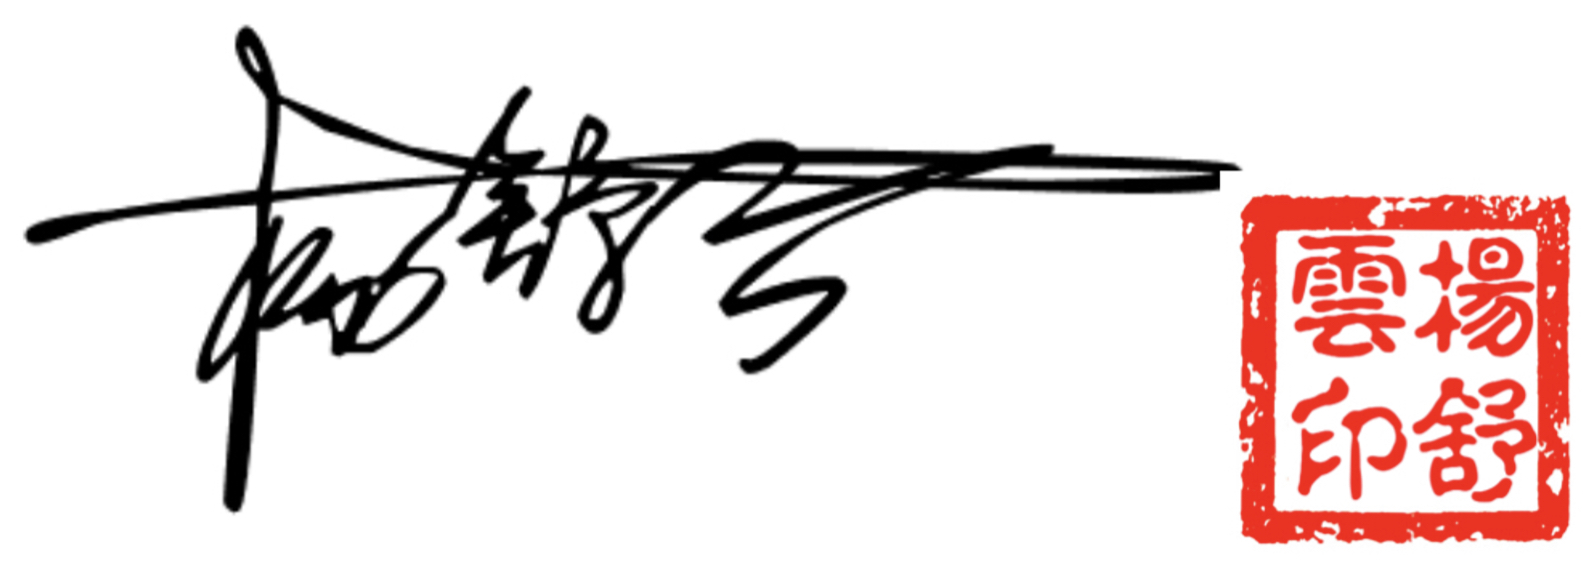
\includegraphics[width=0.45\textwidth]{name.png}
		}
		\subfloat[]{
			
\includegraphics[width=0.45\textwidth]{name-TaLEs.jpg}
		}
		\caption{个人签名}
		\label{fig:name}			
	\end{figure}
	
	% ---
	
	相关代码已上传至Github。
	
	
	
\end{document}